
% This is "sig-alternate.tex" V2.0 May 2012
% This file should be compiled with V2.5 of "sig-alternate.cls" May 2012
%
% This example file demonstrates the use of the 'sig-alternate.cls'
% V2.5 LaTeX2e document class file. It is for those submitting
% articles to ACM Conference Proceedings WHO DO NOT WISH TO
% STRICTLY ADHERE TO THE SIGS (PUBS-BOARD-ENDORSED) STYLE.
% The 'sig-alternate.cls' file will produce a similar-looking,
% albeit, 'tighter' paper resulting in, invariably, fewer pages.
%
% ----------------------------------------------------------------------------------------------------------------
% This .tex file (and associated .cls V2.5) produces:
%       1) The Permission Statement
%       2) The Conference (location) Info information
%       3) The Copyright Line with ACM data
%       4) NO page numbers
%
% as against the acm_proc_article-sp.cls file which
% DOES NOT produce 1) thru' 3) above.
%
% Using 'sig-alternate.cls' you have control, however, from within
% the source .tex file, over both the CopyrightYear
% (defaulted to 200X) and the ACM Copyright Data
% (defaulted to X-XXXXX-XX-X/XX/XX).
% e.g.
% \CopyrightYear{2007} will cause 2007 to appear in the copyright line.
% \crdata{0-12345-67-8/90/12} will cause 0-12345-67-8/90/12 to appear in the copyright line.
%
% ---------------------------------------------------------------------------------------------------------------
% This .tex source is an example which *does* use
% the .bib file (from which the .bbl file % is produced).
% REMEMBER HOWEVER: After having produced the .bbl file,
% and prior to final submission, you *NEED* to 'insert'
% your .bbl file into your source .tex file so as to provide
% ONE 'self-contained' source file.
%
% ================= IF YOU HAVE QUESTIONS =======================
% Questions regarding the SIGS styles, SIGS policies and
% procedures, Conferences etc. should be sent to
% Adrienne Griscti (griscti@acm.org)
%
% Technical questions _only_ to
% Gerald Murray (murray@hq.acm.org)
% ===============================================================
%
% For tracking purposes - this is V2.0 - May 2012

\documentclass{sig-alternate}
\usepackage{comment}
\usepackage{algorithm}
\usepackage{algpseudocode}
\usepackage{multirow}

\usepackage{listings}

%\usepackage[sorting=none]{bibtex}
\newtheorem{theorem}{Jibberish}
\newtheorem{lemma}[theorem]{Lemma}
\newtheorem{proposition}[theorem]{Proposition}
\newtheorem{corollary}[theorem]{Corollary}

\begin{document}


%
% --- Author Metadata here ---
%\conferenceinfo{WOODSTOCK}{'97 El Paso, Texas USA}
%\CopyrightYear{2007} % Allows default copyright year (20XX) to be over-ridden - IF NEED BE.
%\crdata{0-12345-67-8/90/01}  % Allows default copyright data (0-89791-88-6/97/05) to be over-ridden - IF NEED BE.
% --- End of Author Metadata ---

\title{Synthesis of Statically Analyzable Accelerator Networks From Sequential Programs}
%\titlenote{(Produces the permission block, and
%copyright information). For use with
%SIG-ALTERNATE.CLS. Supported by ACM.}}
%\subtitle{[Extended Abstract]
%\titlenote{A full version of this paper is available as
%\textit{Author's Guide to Preparing ACM SIG Proceedings Using
%\LaTeX$2_\epsilon$\ and BibTeX} at
%\texttt{www.acm.org/eaddress.htm}}}
%
% You need the command \numberofauthors to handle the 'placement
% and alignment' of the authors beneath the title.
%
% For aesthetic reasons, we recommend 'three authors at a time'
% i.e. three 'name/affiliation blocks' be placed beneath the title.
%
% NOTE: You are NOT restricted in how many 'rows' of
% "name/affiliations" may appear. We just ask that you restrict
% the number of 'columns' to three.
%
% Because of the available 'opening page real-estate'
% we ask you to refrain from putting more than six authors
% (two rows with three columns) beneath the article title.
% More than six makes the first-page appear very cluttered indeed.
%
% Use the \alignauthor commands to handle the names
% and affiliations for an 'aesthetic maximum' of six authors.
% Add names, affiliations, addresses for
% the seventh etc. author(s) as the argument for the
% \additionalauthors command.
% These 'additional authors' will be output/set for you
% without further effort on your part as the last section in
% the body of your article BEFORE References or any Appendices.

\numberofauthors{0} %  in this sample file, there are a *total*
% of EIGHT authors. SIX appear on the 'first-page' (for formatting
% reasons) and the remaining two appear in the \additionalauthors section.
%
\begin{comment}
\author{
% You can go ahead and credit any number of authors here,
% e.g. one 'row of three' or two rows (consisting of one row of three
% and a second row of one, two or three).
%
% The command \alignauthor (no curly braces needed) should
% precede each author name, affiliation/snail-mail address and
% e-mail address. Additionally, tag each line of
% affiliation/address with \affaddr, and tag the
% e-mail address with \email.
%
% 1st. author
\alignauthor
Shaoyi Cheng \\%\titlenote{Dr.~Trovato insisted his name be first.}\\
       \affaddr{EECS, University of California, Berkeley}\\
       %\affaddr{1932 Wallamaloo Lane}\\
       %\affaddr{Wallamaloo, New Zealand}\\
       \email{sh\_cheng@berkeley.edu}
% 2nd. author
\alignauthor
John Wawrzynek \\%\titlenote{The secretary disavows any knowledge of this author's actions.}\\ 
       \affaddr{EECS, University of California, Berkeley}\\
       %\affaddr{P.O. Box 1212}\\
       %\affaddr{Dublin, Ohio 43017-6221}\\
       \email{johnw@eecs.berkeley.edu}
% 3rd. author
}
\end{comment}
\maketitle
\begin{abstract}
This paper describes a general framework in
transforming a sequential program into a network of processes, which are
converted to hardware accelerators through high level synthesis.
A complementing technique is also proposed to statically analyze the behaviors of the 
generated accelerator network.
The interactions between the accelerators' schedules, the capacity of communication
channels in the network and the memory access mechanisms are incorporated
into our model, such that potential artificial deadlocks can be detected and resolved \textit{a priori}.

An algorithm optimized for FPGA implementation is then developed and applied through our transformation framework. A set of irregular computation kernels are converted into networks of accelerators on FPGA. 
Compare to hardware accelerators generated without going through our transformation, the
accelerator networks achieve significantly better performance.



\end{abstract}

% A category with the (minimum) three required fields
%\category{H.4}{Information Systems Applications}{Miscellaneous}
%A category including the fourth, optional field follows...
%\category{D.2.8}{Software Engineering}{Metrics}[complexity measures, performance measures]

%\terms{Theory}

\keywords{high level synthesis, process network, system design flow,  parallelism, hardware accelerator}

\section{Introduction}
As the growth of processor clock frequency came to a stop in the middle of the last decade, the performance boost provided by the continuous advancement of hardware technology for sequential programs could no longer be sustained. The benefits of user transparent CPU architecture optimizations were also diminishing. With the recent advent of FPGA SoCs~\cite{chips:zynq}, offloading computation to hardware accelerators becomes a promising alternative for
achieving better system efficiency. However,
%To create good implementation in the spatial computing
%paradigm however, is far less intuitive compare to imperative programming.
there is a big gap between the inherently parallel mode of operation in hardware accelerators and the intuitive imperative programming paradigm. Even with tool flows like
high level synthesis (HLS), substantial user inputs are still required to create
efficient implementations~\cite{7082747}. To address this problem, we envision a two
step process, where the sequential specification provided by the user is first
transformed to a more parallel representation, from which the conventional HLS
can easily create high performance compute engine.

\begin{comment}
As parallel computers and more recently, heterogeneous computing platforms become mainstream, it becomes more and more challenging to bridge the gap between the intuitive imperative programming paradigm and the underlying compute substrate.  
In the context of building hardware accelerators on FPGA accelerator
One solution is to leverage more user input, which explicitly specifies the parallelism or


Various parallel programming models were developed with the expectation of users explicitly specifying parallelism in the code. There are also tool chains which converts sequential code to 
hardware accelerators on FPGAs, but more often than not, the big 
\end{comment}

%In this paper, we explore the transformation from sequential programs to networks of processes.
In this paper, we explore this approach by using a modified version of process network (PN), a parallel model of computation, as the target representation for our transformation.
Using FPGA as the computing device, our final implementations are accelerator networks optimized to achieve high throughput in the presence of long data access latency.
Our major contributions include:
\begin{itemize}
    \item We devise a general approach for converting a sequential program to a network
of concurrent processes. Different algorithms can potentially be plugged into the flow, splitting computations between processes in different ways, optimized for the underlying computing substrates.
    \item With FPGA as our target platform, processes are to be converted to hardware accelerators. We
    propose an analysis framework to statically detect and resolve deadlocks in the accelerator networks, ensuring the correctness of the execution. 
    \item We develop an algorithm to generate instances of process networks
particularly amenable to hardware acceleration. Using high level synthesis (HLS), we mapped them onto FPGAs
to demonstrate the benefits of our approach. 
\end{itemize}

\begin{comment}
high level synthesis is used as the final backend to automatically create networks of hardware accelerators. To prevent artificial deadlocks in the final implementation, a
analysis technique was created to reason about the properties of the accelerator network. 

The instruction/loop level parallelism
within each synthesized accelerator, and the coarse grained parallelism between different processes/accelerators can both exploited simultaneously, resulting in great
performance improvement. 
\end{comment}

The rest of the paper is organized as follows:
Section~\ref{pre} provides preliminaries in process network
%intermediate representation of the sequential program,
and accelerator generation using HLS. Section~\ref{mainConvert} describes the main steps in transforming sequential programs
to networks of processes. When implemented on FPGAs, these networks may experience deadlock issues, which can be analyzed and resolved with the method developed in section~\ref{deadlock}. To make our general approach more concrete, we presents a specific algorithm which fits into our PN generation framework in section~\ref{exampleAlgo}.
This algorithm and its complementing optimizations are developed with FPGA as the target platform, thus the generated networks boast great performance when mapped onto the intended 
computing substrate (section~\ref{expEval}). Finally, related work is presented in section~\ref{relatedwork}, before we conclude the paper with discussion and future directions (section~\ref{conclude}).


\section{Preliminaries}
\label{pre}
\begin{comment}
A typical program written for processor execution 
is sequential in its semantics. Techniques to
parallelize this specification need to preserve
the resultant behaviors of the original ordering
of the computation and data access operations.
In this work, we limit the scope of our study
to functions implemented in imperative
languages who terminate in finite time, so that
empirical comparisons can be made. Our approach
tries to transform functions to a different 
model of computation, process networks, before
their
actual implementation on physical computing devices.
\end{comment}

\subsection{Process Networks}
\label{pre1}
The process network, or Kahn process network~\cite{gilles1974semantics}, is an inherently
parallel model of computation where processes communicate with
each other through unbounded FIFO channels. 
The processes cannot test for availability of data tokens in 
the channels without consuming them. If a channel is empty
the process blocks as it reads from the channel.
Writing to the FIFOs, however, is non-blocking.
In addition, each FIFO can only be consumed by a single process, and be written to by a single process. The PN model is deterministic in the sense that the scheduling of
the process execution does not alter the final results. This gives great flexibility
in implementing/controlling each individual processes. 

A characteristic of PN is that all data exchanges are performed over the FIFOs and the notion of a shared global memory does not exist. A program executing on 
a processor however, always have instructions communicating with each other temporally using
the memory. In this work, we bridge this difference by modeling data access as inter-process communication.
%such that our deadlock analysis can also take into account the accelerators' interaction with the memory. 
More specifically, the memory, and its associated interconnect can be seen as a special process which takes in address/data tokens and produces data/acknowledge tokens. In the case where multiple memory ports are exposed, this ``process" does not block on read, as it can choose to serve any port with valid
requests. This behavior is similar to the ``select" function in YAPI~\cite{Kock00yapi:application}, which introduced non-determinism. In our framework however, the non-determinism is addressed by a set of special mechanisms, which will be explained in section~\ref{mainConvert:mem}.


Another necessary deviation from the ideal PN model lies in the capacity of the channels.
In any practical implementations of process network, the FIFOs cannot be unbounded. 
Consequently, writes may block and deadlocks can potentially happen. 
These are so-called artificial deadlocks, as their occurrence is introduced by the nonideality of the implementation and the circular dependency formed %in these deadlocks 
always contain operations writing to a full FIFO.
%Note the memory ``process", which does not block on reads,
%can block on writes (responses to other processes), when a large amount of data returned are not consumed promptly. It may therefore also contribute to the development of artificial deadlocks. 
In a process network, % generated from a sequential program, 
these deadlocks, if left unresolved, would cause a mismatch between
the resultant behavior of the original code and the network. This issue is addressed by our
analysis technique described in section~\ref{deadlock}. 

\begin{comment}
\subsection{Intermediate Representation for Sequential Programs}
Our PN generation flow is built on top of the LLVM framework~\cite{Lattner:2004:LCF:977395.977673}, which uses a single static assignment (SSA) intermediate representation (IR). 
A typical function in a sequential program is represented with
a control flow graph. This is a two level hierarchical structure. Instructions are contained within basic blocks who are connected by directional edges representing control transfers. 
Meanwhile, every instruction defines a new variable in SSA, thus the dataflow between instructions are explicit and well defined.  
\end{comment}



\subsection{High Level Synthesis of Accelerators}
\label{pre2}
A typical HLS tool attempts to capture parallelism in a function written with high level languages like C/C++. With the help of various user provided guidance, it generates hardware in the form of RTL.
Compute operations and data accesses are allocated and scheduled according to the dependency constraints extracted from the input program, and the resource constraints imposed by the target platform. The circuits generated usually follow a Finite State Machine with Datapath (FSMD) paradigm. Activation of a particular operator in the datapath is associated
with a certain clock cycle and the execution of the computation engine is orchestrated by a synthesized central controller. 

With this static scheduling of operations, the accelerators' runtime behavior is rather simple. Different parts
of the generated circuit run in lockstep with each other, no dynamic dependency checking mechanisms,
such as scoreboarding or load-store queueing, are needed.
This rigid scheduling of operators, while producing simpler hardware with smaller area,
is also vulnerable to stalls introduced by cache misses or variable latency operations. This often results in suboptimal performance when the accelerators
are mapped onto FPGAs. The algorithm in section~\ref{exampleAlgo}, was developed to
specifically deal with this issue. Thus the networks generated with the algorithm, when implemented physically, have much better performance. 

\begin{comment}
Depending on the system architecture, the generated hardware can have
different mechanisms in accessing the memory.
In some systems, direct memory access(DMA) engines are instantiated and data movements are explicitly managed, while 
%In the context of a CPU+accelerator system, 
in others, the generated
hardware is presented with a memory interface rather similar to that used by a processor, with various
caching schemes~\cite{6239785}~\cite{6239808} proposed to complement the datapath.

the HLS tools statically schedule
operations when generating accelerators, whose runtime behavior
is therefore rather simple. 

talk about cdfg ssa
process network
\end{comment}

\section{From Sequential Program to Process Network}
\label{mainConvert}
Our PN generation flow is built on top of the LLVM framework~\cite{Lattner:2004:LCF:977395.977673}, which uses a single static assignment (SSA) intermediate representation (IR). 
A typical function in a sequential program is represented with
a control flow graph (CFG). This is a two level hierarchical structure. Instructions are contained within basic blocks who are connected by directional edges representing control transfers. 
Meanwhile, every instruction defines a new variable in SSA, thus the data dependencies between instructions are explicit and well defined.  
%The CDFG representing a function is a hierarchical structure.
%Instructions are contained within basic blocks, which are
%connected by directional control edges. 
To generate process
network from this representation, a few main steps are performed:
\begin{itemize}
\begin{comment}
\item \textit{Branch Predication:} The hierarchy in the IR is flattened by branch predication.
The original control transfers are converted to dependency edges 
between branches and other compute/data access operations. 
\end{comment}
\item \textit{Dependency Annotation:} The hierarchy in the IR is flattened by branch predication. Ordering of memory operations is also enforced by the addition of
special dependency edges into the graph.

\item \textit{Instruction Cluster Formation:} The instruction nodes, with various dependencies between
each other, are partitioned into multiple sets. This is the core part of the flow. Different algorithms targeting compute substrates of different characteristics can be applied in this step. 

\item \textit{CFG Reconstruction:} From each set of instruction nodes, a CFG is reconstructed
to form a self-containing process. Dependencies between the instruction
nodes are realized by the communications between the recreated CFGs. 
\begin{comment}
\item \textit{Accelerator Network Generation:} The reconstructed CDFGs are pushed through
high level synthesis, producing an array of communicating hardware accelerators. Linked together
by FIFO channels, these concurrently executing modules form a network which is functionally
equivalent to the original sequential specification.
\end{comment}
\end{itemize}

%\subsection{Branch Predication}
\subsection{Dependency Annotation}
\label{mainConvert:mem}
To facilitate the instruction partitioning, we perform predication to eliminate the basic block boundaries, creating a unified graph of nodes with the
addition of control dependency edges. 
The simplest way to insert these edges is to have every instruction dependent on the last branch of the immediate
predecessors of its container basic blocks. However, we take a more aggressive approach, looking for the earliest control transfer which necessarily leads to the execution of an instruction.
Given an instruction $i$ and its container basic block $bb$, our
flow looks for the nearest set of basic blocks $BB'$ who are not properly post-dominated by $bb$,
and insert the dependency edge between the branch instructions ending each member of $BB'$ and $i$. Compare to the naive predication, this approach use a single control edge to replace a sequence of edges traversing multiple branches, reducing the overall communication
overhead in the network. Also with the elimination of unnecessary edges, the subsequent steps can be more flexible, potentially leading to more efficient final implementation.

Another type of dependencies is implicitly carried by memory accesses. When
two memory accesses target the same location and one of
them is a store, their order in the original program execution
needs to be preserved--a dependency edge is added
between them. We try to avoid adding unnecessary edges as they
can potentially affect the instruction partitioning negatively. 
The flow currently relies on alias analysis to perform partitioning of the memory space. No edges are inserted for accesses to disjoint memory partitions. 
Meanwhile, for code harder to analyze, the flow can take in user annotations, complementing the overly conservative compile time analysis. 

With the addition of these edges, the ordering of requests sent to the memory
subsystem is constrained to be consistent with the original program execution.
The non-determinism caused by memory selecting amongst multiple requests no longer
impacts the final outcome. In general, for any pair of instructions separated into two sets, the necessary ordering between them is enforced by the cut edges,
which will eventually be converted to communication channels between processes.

\subsection{Instruction Cluster Formation}
\subsubsection{Partitioning Instructions}
To create multiple processes, the instruction nodes are to be distributed into multiple sets. The actual partitioning of instruction nodes can use different algorithms, targeting compute substrate of different characteristics. In our implementation, a predefined interface is created, which takes in a fully annotated dependency graph and outputs separate collections of instructions. These can then be fed to the next stage of our flow. This is 
a convenient way to experiment with various techniques, leveraging other parts of the framework to reconstruct processes, detect/resolve deadlocks and generate concrete implementation. For instance, the decoupling method described in~\cite{dswp} can be easily plugged into the flow, generating network optimized for multicore processors. We have also developed our own algorithm targeting FPGAs, which is detailed in section~\ref{exampleAlgo}. 
There may even be scenarios where work can be divided up amongst FPGA accelerators and CPUs, requiring the partitioning routine to consider characteristics of multiple platforms simultaneously. For any of these cases, our infrastructure
can be used with minimal change.

\begin{comment}
However, before this partitioning can happen, more information needs to be added to the graph. Specifically, there are dependencies
implicitly carried by memory accesses. When
two memory accesses target the same location and one of
them is a store, their order in the original program execution
needs to be preserved--a dependency edge is to be added
between them. We try to avoid adding unnecessary edges as they
can potentially affect the instruction partitioning negatively. 
The flow currently relies on alias analysis to perform partitioning of the memory space. No edges are inserted for accesses to disjoint memory partitions. 
Meanwhile, for code harder to analyze, the flow can take in user annotations, complementing the overly conservative compile time analysis. 

With the addition of these edges, the ordering of requests sent to the memory
subsystem is constrained to be consistent with the original program execution.
The non-determinism caused by memory selecting amongst multiple requests no longer
impacts the final outcome. In general, for any pair of instructions separated into two sets, the necessary ordering between them is enforced by the cut edges,
which will eventually be converted to communication between processes.

For every pair of operations whose ordering needs to be preserved, a special dependency edge is added between them. Since the generation of the sets is performed around strongly connected components in the original dataflow, it is important to avoid adding unnecessary memory dependency edges. To achieve this, our flow currently relies on alias analysis to perform partitioning of the memory space. Accesses to disjoint memory regions can be safely reordered. When the source code contains pointer arithmetic or irregular memory accesses, compile time alias analysis may produce overly conservative results, in which case user annotations can be used to provide hints to the tool, similar to~\cite{manycache}. This partitioning of memory space naturally leads to creation of multiple data access interfaces, whose interactions with the memory subsystem can be customized, as will be elaborated in section~\ref{sec:optmem}.  


Under certain circumstances, we do not want to directly add edges between memory operations
as they hinder the CDFG partitioning. For the example in figure~\ref{fig:barrier}, during the execution of one outer loop iteration, the set of memory addresses accessed by the the load does not intersect
with that of the store instruction. However, across different outer loop iterations, these
two instructions can accesses the same locations. 
We can conservatively make them dependent
on each other, but this creates an SCC that ultimately prevents any partitioning, as can be
seen in the figure.



%become the performance bottleneck. 
Alternatively, a memory barrier can be inserted after the completion of 
each outer loop iteration. To implement the barrier in the pipeline, the stage containing
the semantically earlier instruction sends tokens to stages who contain the successor
instructions. Eventually during the RTL generation, the local schedule of instructions also needs to be constrained such that the sender of the barrier tokens is not reordered to before its predecessors, while the receivers execute before its semantic successors as well.

The insertion of the sender/receiver of the barrier happens after the instruction partitioning. Depending on if a partition is the sender or receiver of the token,
an extra store/load operation is introduced into the set of instructions, associated
with the basic block where the barrier occurs.
\end{comment}

\subsubsection{Optimizing Communication v.s. Computation}
\label{opt}
 Regardless of exactly how the instructions are partitioned, as each process performs its computation locally, the necessity to communicate with its peers can incur implementation overheads.
For each communication channel, buffer space is to be allocated, and sender/receiver primitives also need to be inserted. Therefore, it is sometimes beneficial to duplicate some nodes after the instruction partitioning. Given sets of instruction nodes created after applying a platform-specific algorithm, for each of these set $G$, the problem of whether to copy other instruction nodes into $G$ can be formulated as an integer programming problem. 

Let $T$ be the set obtained with nodes duplicated into $G$, and the set of remaining nodes be $S$. Each node $i$ can be associated with a binary variable $p_i$, where $p_i = 0$ if $i \in T$ and $p_i = 1$ if $i \in S$. Meanwhile, each edge $ij$ is associated with
a binary variable $d_{ij}$ which takes the value 1 if $i \in S$ and $j \in T$, and 0 otherwise. Finally, $w_{ij}$ is used to represent the cost of edge $ij$
while $c_i$ represents the cost of the node $i$.


\begin{equation}
\begin{aligned}
\label{ilpopt}
& {\text{Minimize}} & & \underset{ij \in E}\sum w_{ij}d_{ij} +  \underset{j \in T}\sum c_j \\
\end{aligned}
\end{equation}
\begin{equation*}
\begin{aligned}
& \text{subject to: }
& &  d_{ij} - p_i+p_j \ge 0, & ij \in E \\
& &  & p_i \in \{0,1\}, & i \in V \\
& & & d_{ij} \in \{0,1\}, & ij \in E \\
& & & p_{G} = 0
\end{aligned}
\end{equation*}

Depending on the implementation platform, the cost of the edges and nodes can be assigned differently. This formulation however, is platform-neutral and generally applicable.
With the CPLEX~\cite{iILO06a} optimization software, this ILP can be solved heuristically and the sets of instructions can be updated accordingly.
%The resulted sets of instructions are then passed to the next stage of our flow.


\subsection{CFG Reconstruction}
%Need fixing
From each set of instructions generated,
an executable process is created by constructing an independent control flow graph. This step recreates basic blocks to in the new CFG, while inserting communication primitives to send and receive tokens through FIFO channels.
\begin{itemize}
    \item For every instruction $i$  in the current set, recreate
    its container basic block if it's not already in the CFG.
    \item For every instruction $j$ on which $i$ depends, 
    recreate its container basic block if it's not already
    in the CFG.
    \item If $j$ is associated with another set of instructions, a load operation
    is created locally as a placeholder in its container basic block.
    \item If $i$ is producing operands for instructions assigned to 
    other sets, a store operation is inserted after $i$.
\end{itemize}
The set of recreated basic blocks $B$ are thus associated with either the instructions assigned to the current set, or the placeholder instruction supplying them with operands. 
%We then proceed to mirror all the relevant execution paths in the original CFG. We .
%$d$ is used as the entry block for our new CFG. Basic blocks in the path from $d$ to
%every basic block $b \in B$ are added to the CFG 
The insertion of load and store operations is to accommodate various
dependencies between the processes. Note each pair of these inserted communication primitive is associated with a single instruction in the original CFG.The flow of
tokens between them ensures the execution path are synchronized across different CFGs
and the right operands are supplied for computations distributed across the
process network. 

To form execution paths in the new CFG, we find the nearest common dominator $d$ of all the recreated basic blocks from the original CFG. It is added to $B$ and used as the new entry block. Again from the original CFG, we trace all the paths between member basic blocks in $B$, and add the points of divergence into $B$. These points are basic blocks which cause
the control flow to go into different members in $B$, or to basic blocks not in $B$ at all.
With these basic blocks connected, we have a self-contained process. 
During this construction process, for the branch instructions not already assigned to the current CFG, a load operation is created to accept a branch target token from another process. The local control flow can then be performed according to this received token. 
Finally, if the entry block $d$ was inside a loop in the original control flow, any branch out of the set $B$ is redirected to $d$. We are essentially enclosing the process with a \textit{while(true)} loop and the execution of the new CFG will be repetitively activated by the availability of the proper tokens.


%FIXME --- no while loop for the last partition
\begin{figure*}[htp]
\begin{center}
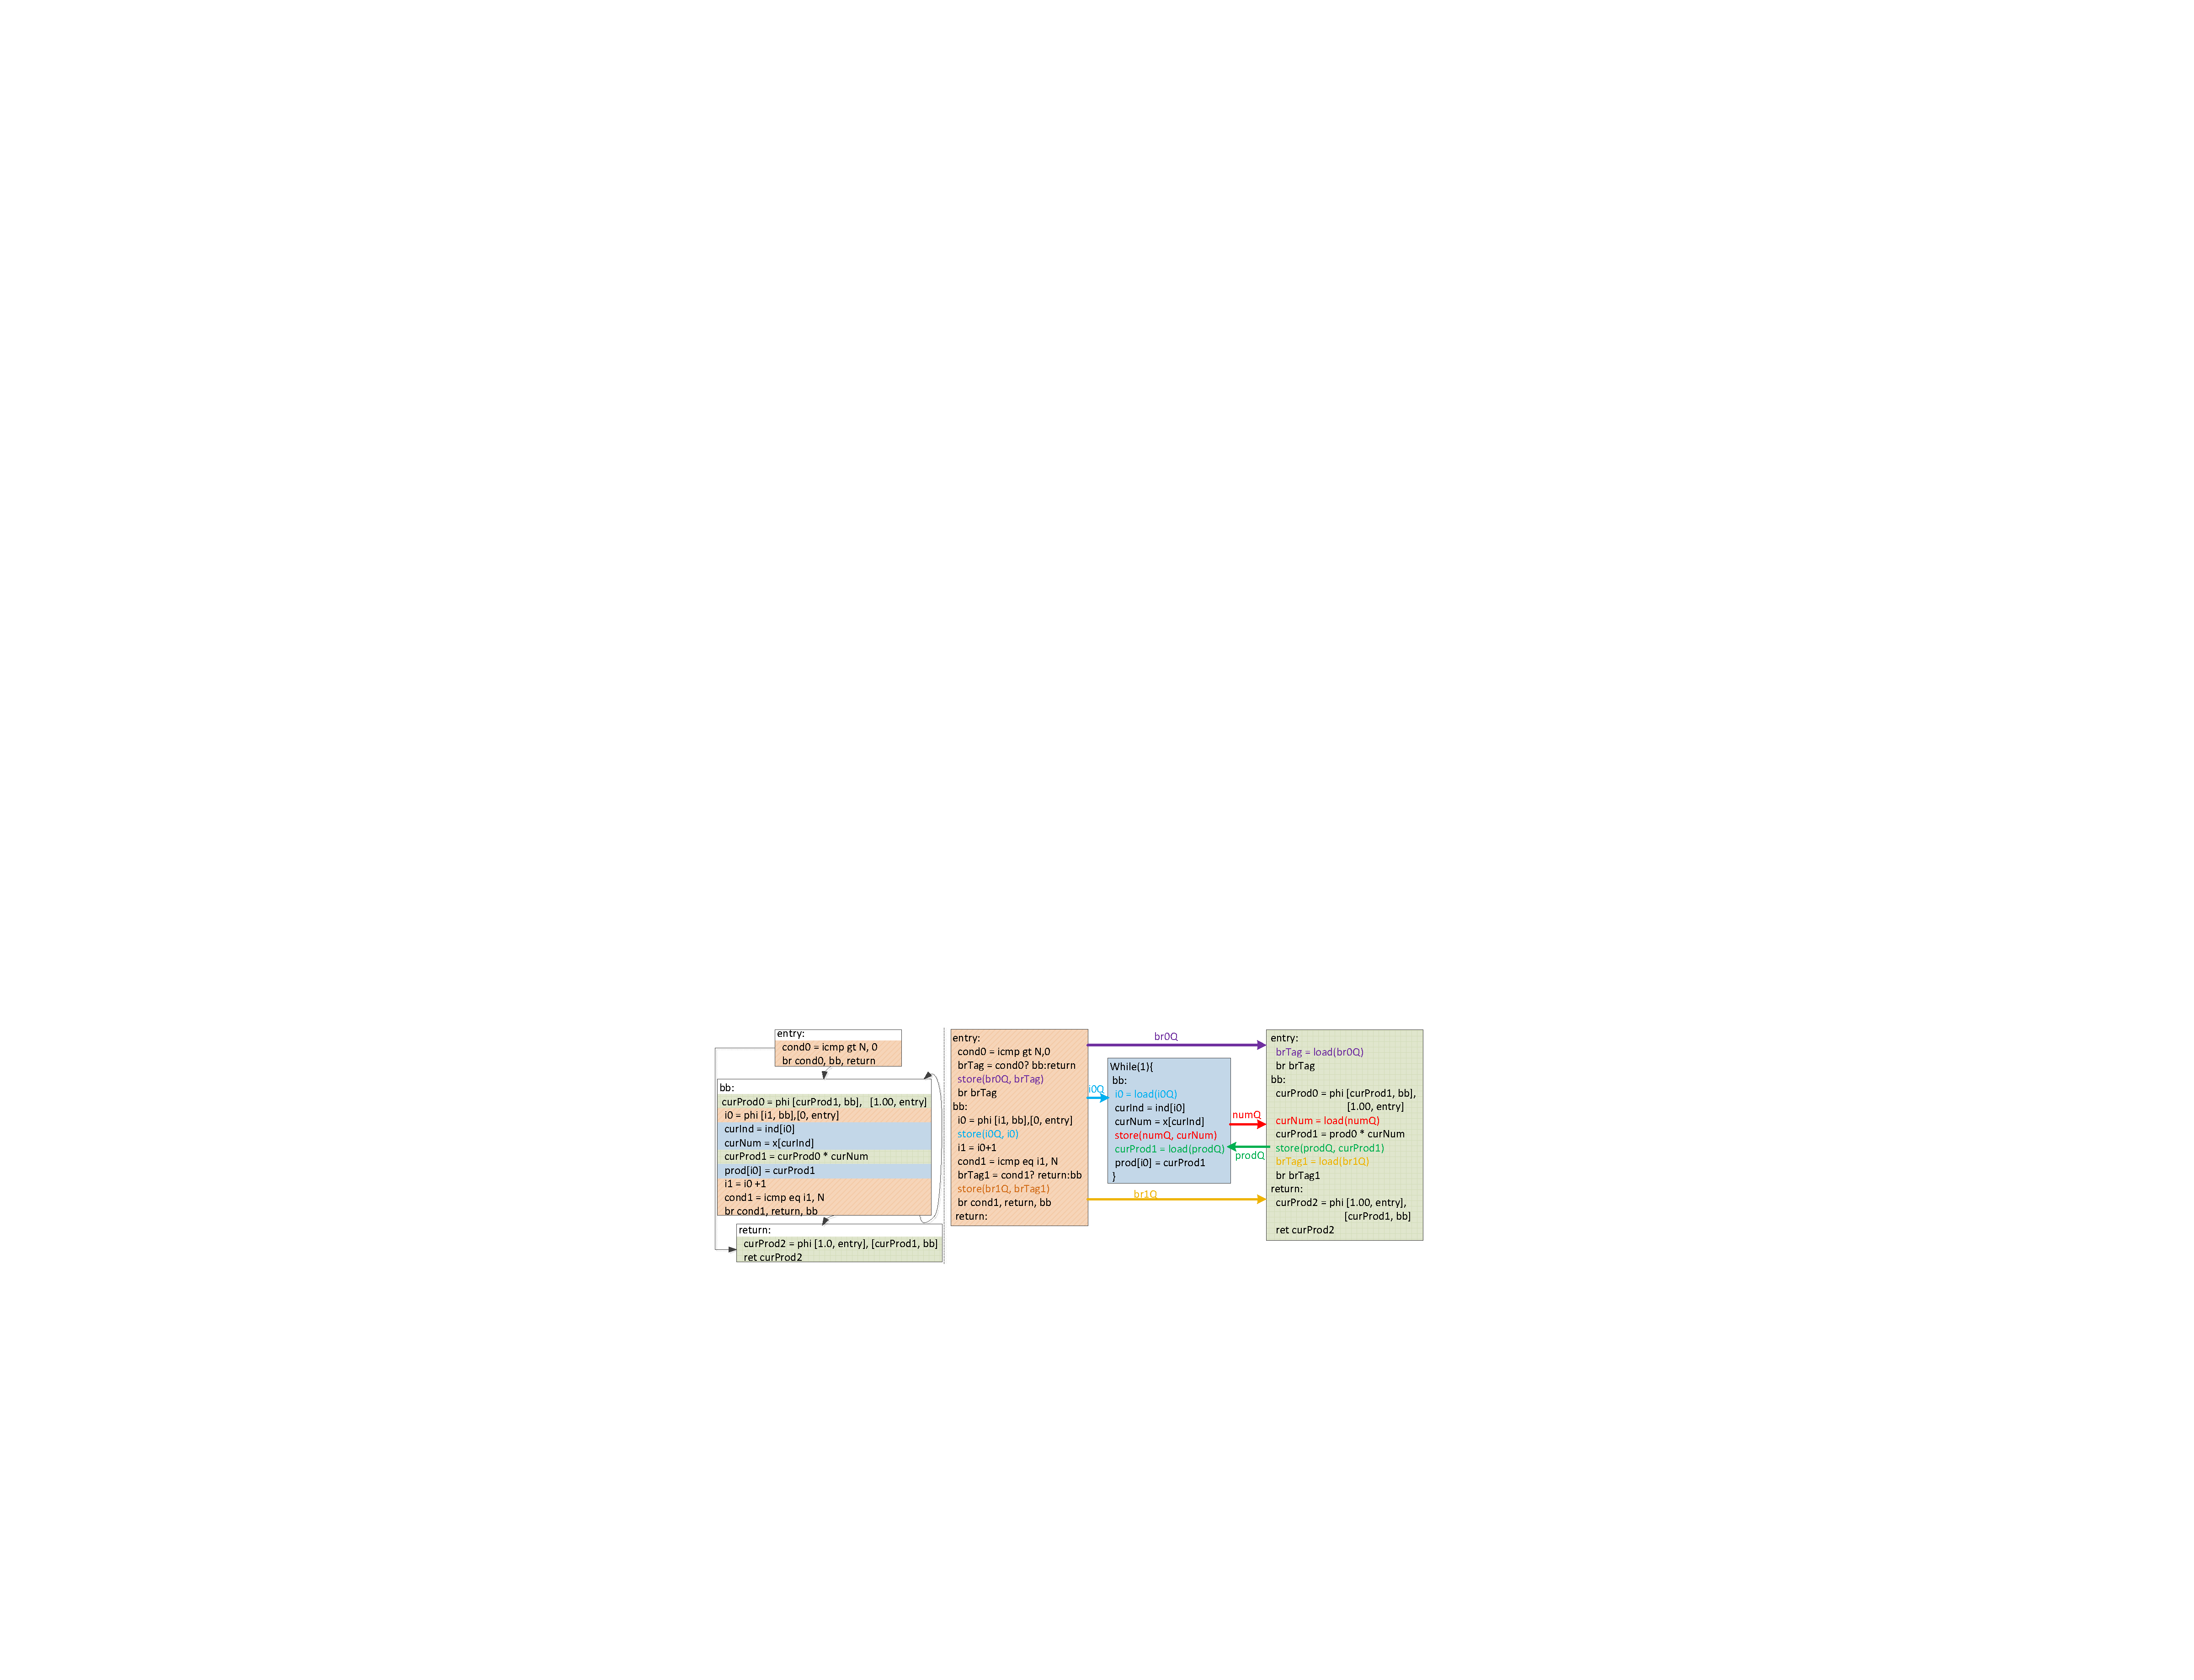
\includegraphics[width=1.0\linewidth]{fig/convert.pdf}
\caption{From A Single CFG to A Process Network
\label{fig:totalFlow}}
\end{center}
\vspace{-2.0em}
\end{figure*}

In figure~\ref{fig:totalFlow}, the function below is converted from its SSA form to a process network.  A naive instruction partitioning algorithm is used in this example. The loop control flow, the memory access and the computation are separated into three different
processes.

\begin{comment}
To mirror the relevant execution path in the original program, a few more steps need to be taken.
\begin{itemize}
    \item In the CFG of the original program, find the nearest common dominator $d$ of all the recreated basic blocks $B$, and add $d$ to $B$. It will be the entry block of our new CFG.
    \item Find all the paths $P$ from $d$ to $b \in B$, add all the 
    basic blocks in each $p \in P$ to $B$.
    \item From each $b \in B$, find the paths $P_b$ to every $b' \in B$ without passing through $d$. Add all the basic blocks in each $p_b \in P_b$ to $B$. \item Create the branching instructions at the end of each $b \in B$. If the branching instruction was already assigned to the current CFG, nothing needs to be done, otherwise a load operation is created to accept
    a branch target token from another process, and then the actual branching is performed according to the received token. 
    \item 
\end{itemize}
\end{comment}

\begin{lstlisting}
float foo(float* x, float* prod, int* ind)
{
  float curProd = 1.0;
  for(int i = 0; i < N; i++){
    int curInd = ind[i];
    float curNum = x[curInd];
    curProd = curProd * curNum;
    prod[i] = curProd;
  }
  return curProd;
}
\end{lstlisting}
When this network runs, it writes the same data into the memory, and eventually return
the same value as the original program. As it completes execution, its processes will either return or be blocked on empty FIFO. However, whether it can successfully complete hinges on
the absence of artificial deadlocks, which we are going to look at next.

\begin{comment}
During the execution, the same data 
When it runs,  returns the same value, and writes the same data into the memory as the original program, assuming no artificial deadlock occurs. 

In the control flow graph of the original program, the set of paths whose starting points and end points both fall in $B$ can be divided into
two groups. Some of these paths never reach basic blocks outside of $B$, and the rest go out of $B$ and then come back into $B$ via $d$. 
The first group
is completely contained within our CFG.  If there is any path in the second group, then $d$ must be inside a loop, in which case we have effectively enclose the CFG with a \textit{while(true)} loop and the execution of the part
of the path within the CFG will be repetitively activated by the availability of the proper tokens.
\end{comment}




\begin{comment}
The insertion of load and store operations is necessitated by various
dependencies between the processes. The flow of
tokens ensures the execution path are synchronized across different CFGs
and the right operands are supplied for computations distributed across the
process network.
\end{comment}





\section{Artificial Deadlock Analysis}
\label{deadlock}
\subsection{Boundedness of the Generated PNs}
As mentioned in section~\ref{pre1}, it is impossible to have unbounded communication FIFOs between processes in any real PN implementations. For a PN to execute without experiencing artificial deadlocks, it has to be bounded, i.e. certain schedule of the network only requires finite FIFO space.
For a general PN, its boundedness is an undecidable problem~\cite{parks1995bounded}. However, for the process networks generated using our scheme, 
%we can first show it is possible to execute within bounded space, and
%then find the FIFO space necessary to ensure the absence of artificial deadlocks. 
we can easily show their boundedness by constructively create a schedule of operations.

The main observation here is that for every token sending instruction, there is a corresponding token consuming instruction. Furthermore, they both derive from the same instruction in the CFG before partitioning. Therefore, we can create a schedule $H$ for our network following the execution of instructions in the original program. For every instruction executed in the original CFG, we schedule the PN's instructions derived from it in $H$. If these instructions are involved in communication, the source of the data tokens is scheduled first, immediately followed by the token sinks. It should be apparent that only one slot is needed
in each communication channel for the process network to execute, since the produced tokens are promptly consumed.

\subsection{Instruction Schedules and Deadlocks}
Now let the schedule of instructions in each process $p$ be $G(p)$, we say $G(p)$ is \textit{locally consistent} with $H$ if and only if 
$\overline{i_a} \prec \overline{j_b}$ in $H$ $\Rightarrow$ $i_a \prec j_b$ in $G(p)$
, where $\overline{i_a}$, $\overline{j_b}$ are invocations of instructions in $H$, and $i_a$, $j_b$ are their equivalences in $p$. 
\begin{lemma}
\label{nondeadlock}
Assuming 
%requests to $M$ is first-come first-served,
all FIFOs are of size one,
as long as $G(p), \forall p \in PN$ are locally consistent with $H$,
artificial deadlock will not occur in $PN$. 
\end{lemma}

Assume there is an artificial deadlock, we can go around the dependency
cycle and examine the blocked processes $P_b \subseteq PN$. For a process $p_b$
to be blocked at invocation of instruction $j_0$, $j_0$ is either reading from an empty FIFO, or writing to a full FIFO. For the former case, the FIFO is empty because the token's producer instruction $j_0' \in p_b'$ cannot execute, which indicates an earlier instruction  $i_k'$ in $G(p_b')$ is blocked. For the later case, the FIFO is full because the token produced by an earlier invocation $j_{-1}$ has not been taken by its corresponding consumer instruction $j''_{-1} \in p_b''$. This also indicates an earlier instruction $l_n''$ in $G(p'')$ is blocked. Apply this reasoning recursively around the circle of dependencies,
we should have a chain of precedence among instructions invocations $j_0 \succ i_k' \succ ... \succ j_0$
or $j_0 \succ j''_{-1} \succ l_n'' \succ ... \succ j_0$ in $H$. %As all invocations of instructions in the chains come from schedules locally consistent with a single schedule $H$, 
Both chains are self-contradictory and therefore, the scenario for artificial deadlock can never occur. 

Since $H$ is derived from the original CFG, with Lemma~\ref{nondeadlock} proven, we can conclude that if each of the generated process is executed strictly according to the original program order, we will have a network free from artificial deadlock. This
will guarantee, for instance, when processors are used as the compute substrate, the network will produce the correct result as each process is executed according to locally consistent $G(p)$. On the other hand, when HLS is used to create hardware accelerators from processes, this guarantee may not
hold anymore since aggressive parallelization and reordering of instructions
would violate the consistency between $G(p)$ and $H$. 

%This is illustrated in figure~\ref{fig:example}.
\begin{figure}[htp]
\begin{center}
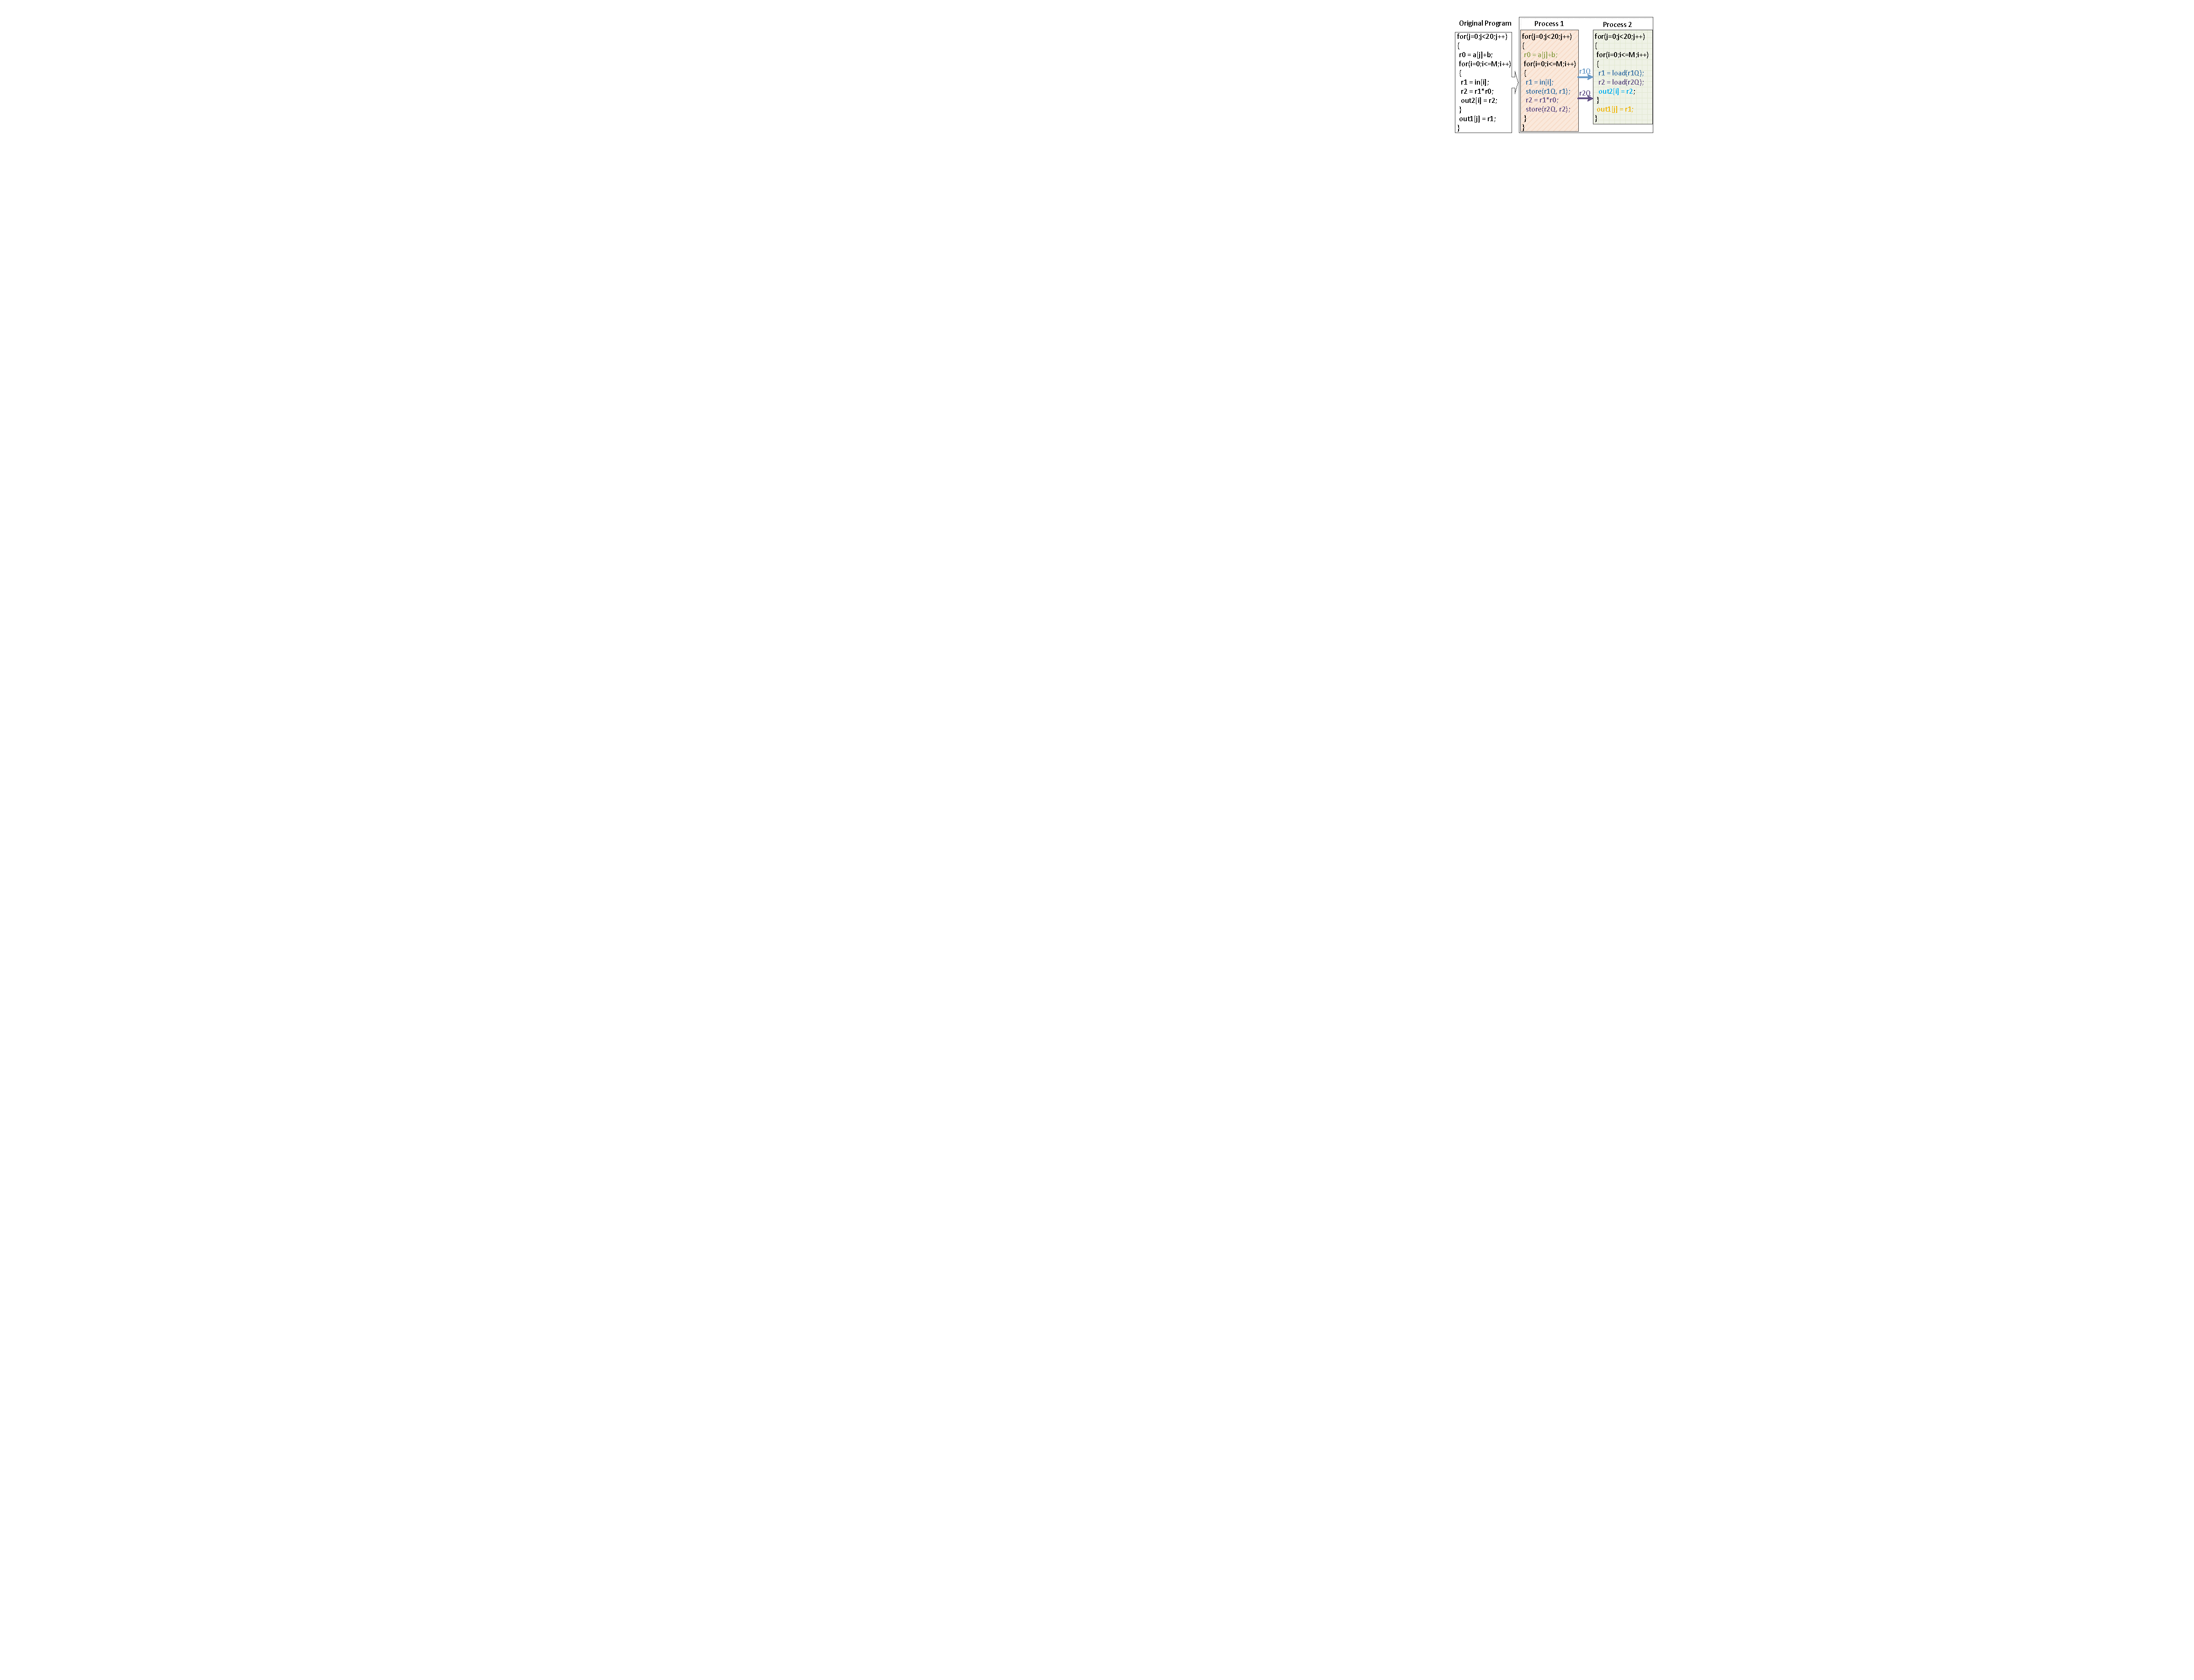
\includegraphics[width=1.0\linewidth]{fig/dlmo.pdf}
\caption{Example PN for Deadlock Analysis
\label{fig:example}}
\end{center}
\vspace{-1.5em}
\end{figure}

\begin{figure*}[htp]
\begin{center}
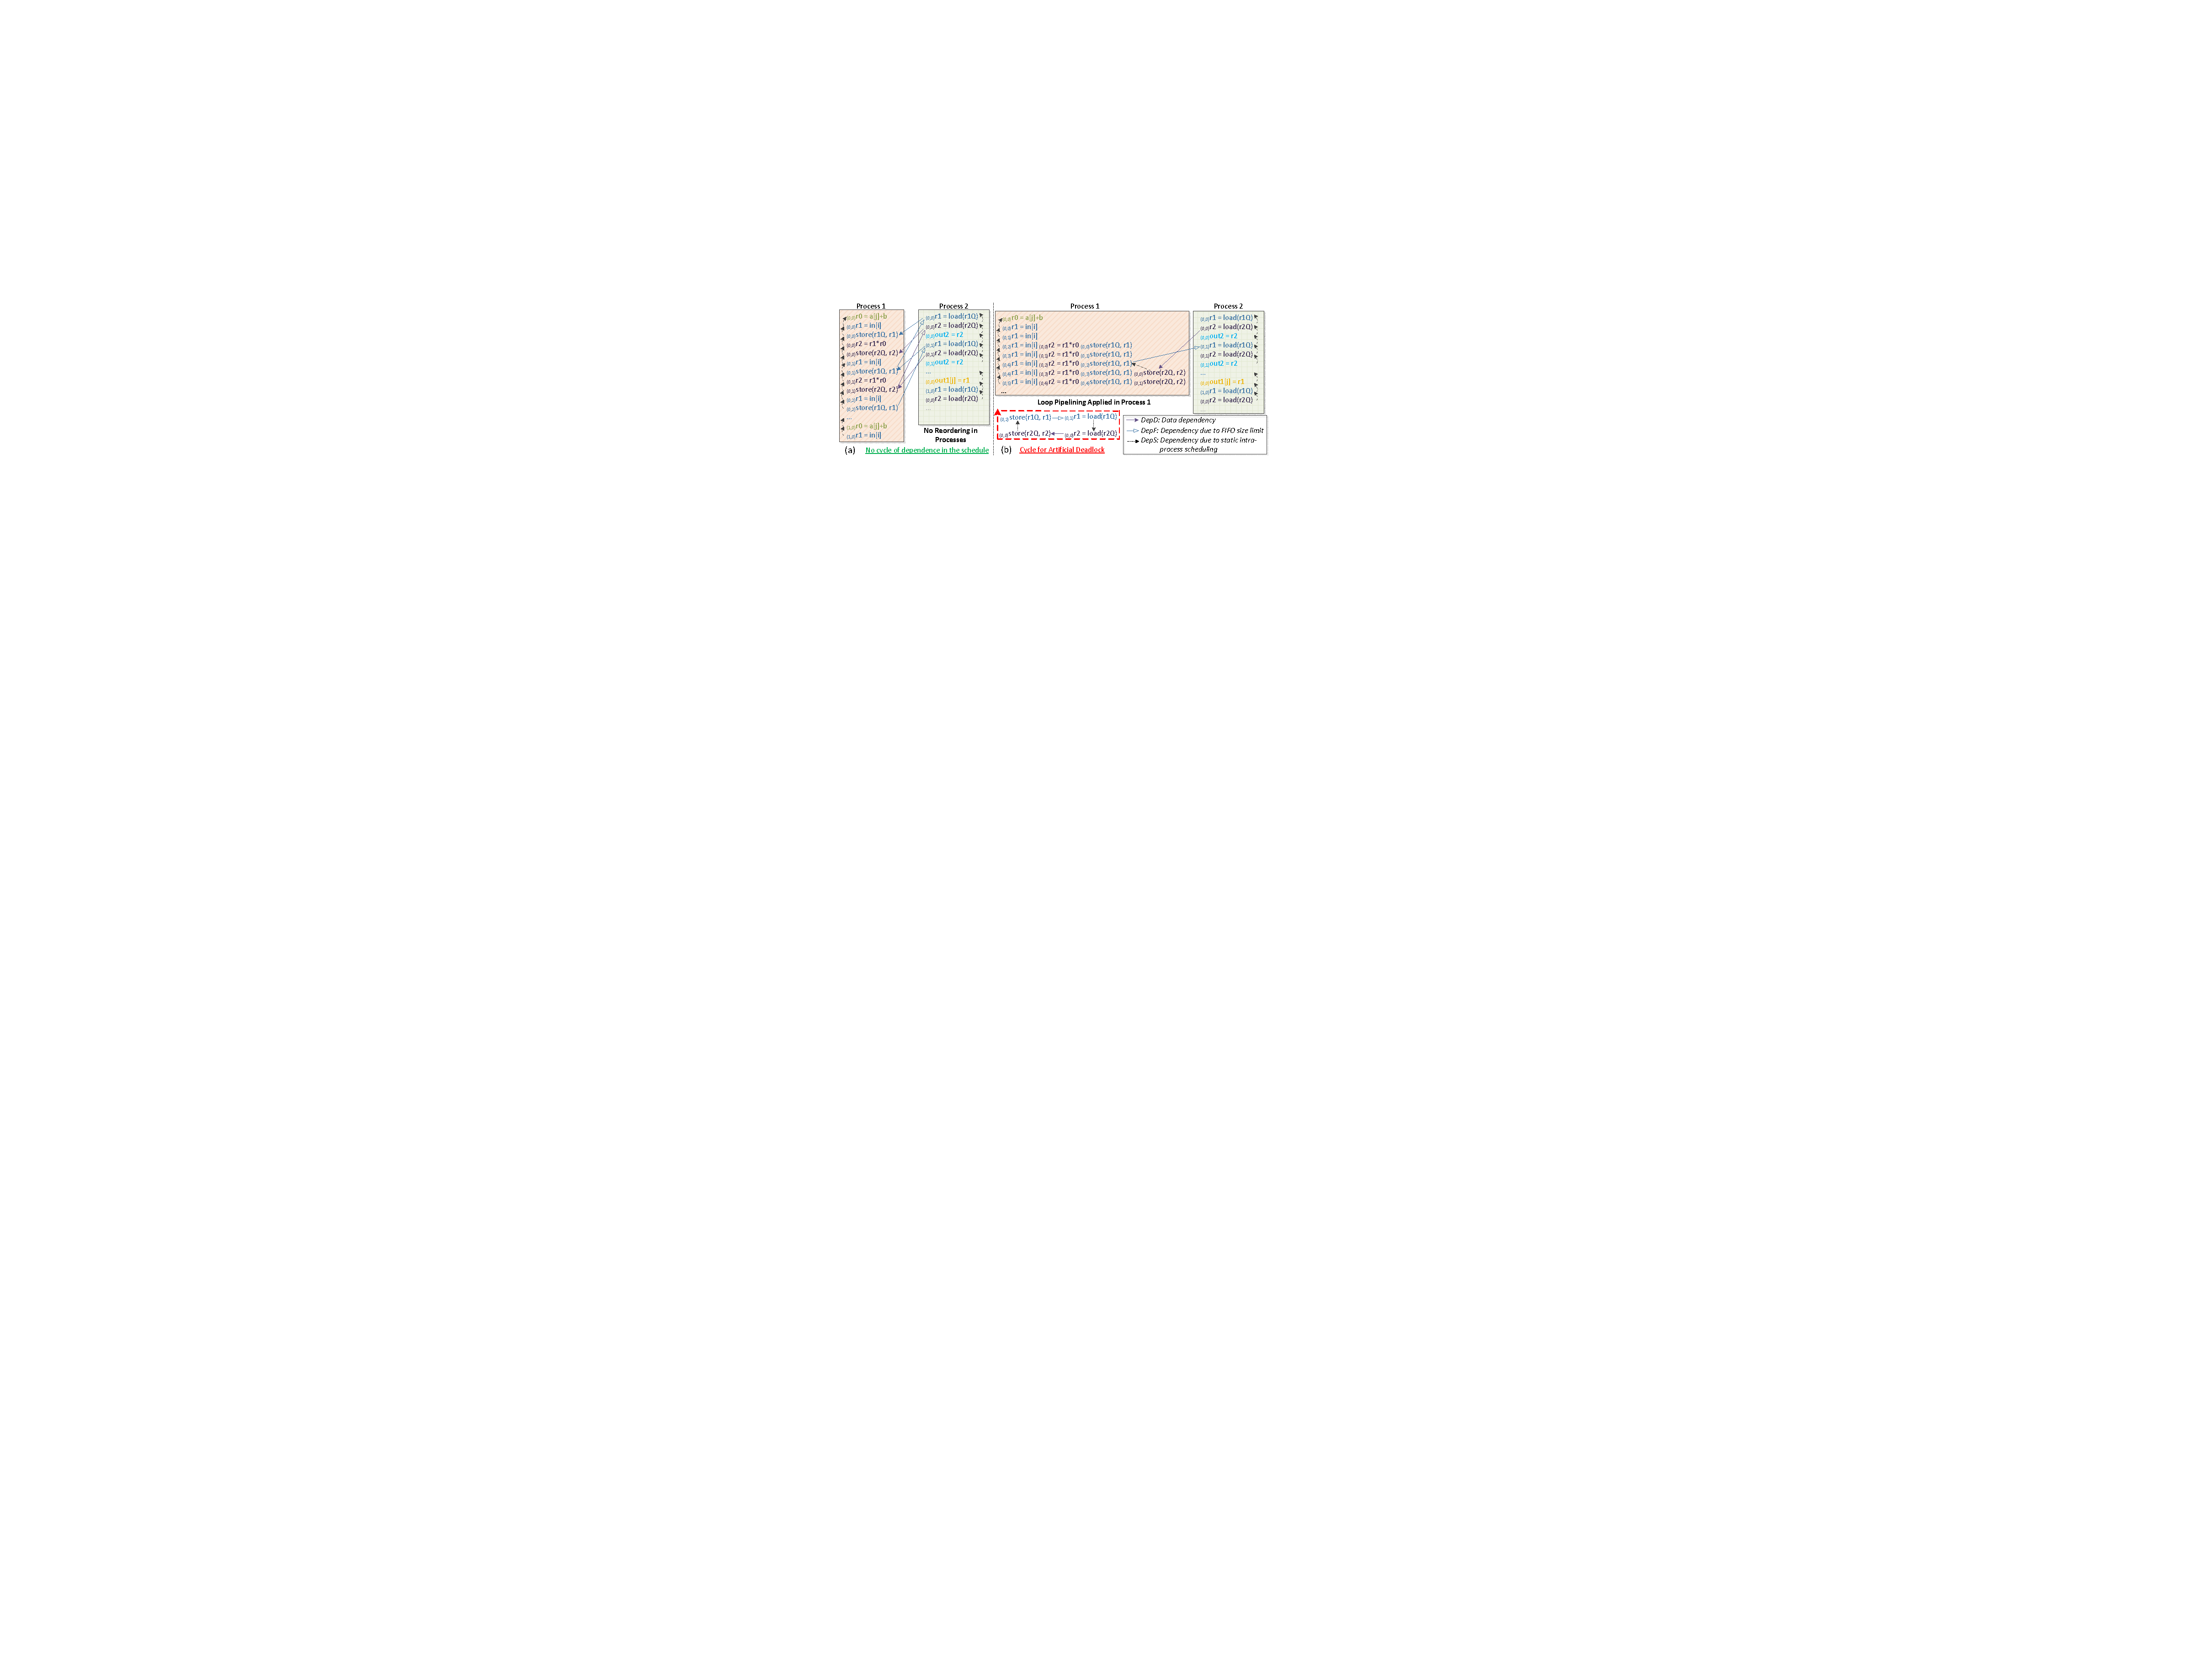
\includegraphics[width=1.0\linewidth]{fig/twoSchedules.pdf}
\caption{(a) No Reordering, No Deadlocks (b) Loop Pipelining Introduces Deadlock
\label{fig:2schedules}}
\end{center}
\vspace{-2.0em}
\end{figure*}

Figure~\ref{fig:example} is a simple generated PN we use to illustrate this problem. The original program is converted to a two process network
with two single slot communication channels between them.
Figure~\ref{fig:2schedules} then shows the scheduling and communication of the processes. Each instruction invocation is prefixed with a vector, representing its place in the (j,i) iteration space, and three types of dependency edges are used
to show the necessary precedence among these invocations. There is no cycle of
dependency in (a), and therefore no deadlocks, when both processes execute in program order. However, in (b), 
a common HLS technique, loop pipelining, is applied to \textit{Process 1}, where
iterations of the loop are aggressively overlapped. Every cycle, a new iteration is started. Because of the long latency of load from \textit{in[i]} and
the multiplication, the sending of the first \textit{r2} token, $_{(0,0)}$store(r2Q,r2), is scheduled
after many instruction invocations for later iterations. Due to the static scheduling, it can not execute until after $_{(0,2)}$store(r1Q,r1), whose
writing to FIFO r1Q cannot happen until the previous token is consumed by 
$_{(0,1)}$load(r1Q). Because of the scheduling in process 2, this load from r1Q
occurs after $_{(0,0)}$load(r2Q), which cannot complete unless $_{(0,0)}$store(r2Q,r2)
can send the token.  An artificial deadlock is therefore created. 

\begin{comment}
This fixed, highly parallel schedule of instruction invocations 

The actual scheduling of instruction invocations are then shown in figure~\ref{fig:2schedules}. 

%shows a simple example of a otherwise deadlock free network becomes problematic.
%In the example, the original program is converted to a two process network
%with two single slot communication channels between them. 
A common technique in HLS, loop pipelining, can start a new iteration of a loop before the previous ones are completed. This results in the rescheduling of operations in process 1. Now a otherwise deadlock free network becomes problematic. Due to the size limit of the FIFOs, which is one in this case, the execution
of the producer instruction is dependent on the completion of the previous invocation
of the consumer instruction. In figure~\ref{fig:example}, as the instructions in process 1 is statically reordered, a circular dependency is formed
between instructions: INS $B_1$ cannot execute unless
INS $A_4$ completes, and INS $A_4$ cannot execute until
INS $A'_3$ consumes the token from INS $A_3$. But INS $A_3$ cannot happen until INS $B'_1$ occurs, and
that depends on the completion of INS $B_1$.  An artificial deadlock
is therefore created. 
\end{comment}




%when the instructions are statically reordered in individual processes by HLS. 


The classic approach to resolve artificial deadlock is by increasing the size of the FIFO where write is blocked~\cite{parks1995bounded}. 
In this particular example, if the size of r1Q is increased
from 1 to 2, then the execution of $_{(0,2)}$store(r1Q,r1) would be dependent on 
$_{(0,0)}$load(r1Q) instead of $_{(0,1)}$load(r1Q). The cycle of dependence is broken as there will be no path of dependence from $_{(0,1)}$load(r1Q)
to $_{(0,0)}$store(r2Q,r2). The deadlock no longer exists.

Unfortunately, in a network implemented in hardware, the FIFO size cannot be easily increased.
%As the producer and consumer instruction instances are rescheduled differently with
%respect to other instructions in their own process, blocking write causes
%artificial deadlock. Increasing the number of slots in the FIFO can help resolve
%this problem. 
To determine the needed buffer space in the channels \textit{a priori}, simulations are sometimes used~\cite{buck1994ptolemy}. It relies 
on using representative dataset as input and for certain type of problems, simulation results may not provide any guarantee, especially if the control flow is runtime data dependent. In this section, we want to analyze the interaction between FIFO
sizing and intra-process instruction scheduling, 
so we can better understand
their joint effect on the liveness of the process network.

\subsection{Precedence Graph for Deadlock Detection}
To directly detect cycles from the schedules of processes as we have done in 
figure~\ref{fig:2schedules} is unrealistic as each schedule may contain potentially infinite instruction invocations.
However, HLS tools generate a short, repeatable schedule for each process.
We can leverage it to create a more concise representation--precedence graph.




An example of the precedence graph is shown in figure~\ref{fig:predgraph}, the schedules of instruction invocations are condensed into a small graph whose edges carry vector weights. 
%As illustrated in the figure, in a schedule of a multiple level loop nest, the instruction invocations can be annotated with subscripts representing their position in the iteration space. For instance, instruction executed in the second iteration of the inner loop within the third iteration of the outer loop has subscript (3,2). Also, outer loop instruction
%invocations carry 1 at the position of the vector corresponding to the inner loop level. 
The weights of the $DepS$ edges are simply the worst case differences between the vector prefix of invocations of a pair of instructions. 
Similarly, the $DepF$ edges corresponds to the difference in prefixes between
the consumer and producer instruction invocations. Note this is directly related
to the number of slots in the FIFO. For our example, the edge from store(r1Q,r1) to its consumer load(r1Q) carries a weight of (0,-1) when the channel has just one slot.
It means the previous invocation of the consumer instruction needs to complete before the producer instruction can write more tokens. The $DepD$ edges, on the other hand, always have weight $\vec{0}$ as the consumer depends on the producer with the same iteration vector. In essence, this graph
summarizes the necessary precedence between instruction invocations. 

In the precedence graph, every simple cycle has a weight sum which is also a vector. An deadlock is manifested as a cycle with weight being the zero vector ($\vec{0}$) or vectors whose first non-zero elements (leading elements) are positive.
They indicate an instruction invocation depending on itself or a later invocation in the execution, and thus a deadlock. 
The computation to find deadlocks may potentially be expensive. In the worst case, the number of simple cycles in the graph can be exponential in
$|V|$, the number of nodes in the graph. However, practically, the number of
nodes involved are approximately the same as the number of channels needed, as
we only need to look at the loads and stores from/to FIFOs.
The graph is also rather sparse in the connectivity between these nodes.  
Methods such as~\cite{doi:10.1137/0204007} can be used for efficient
enumeration of the cycles and the subsequent identification of the deadlocks.


\begin{figure}[htp]
\begin{center}
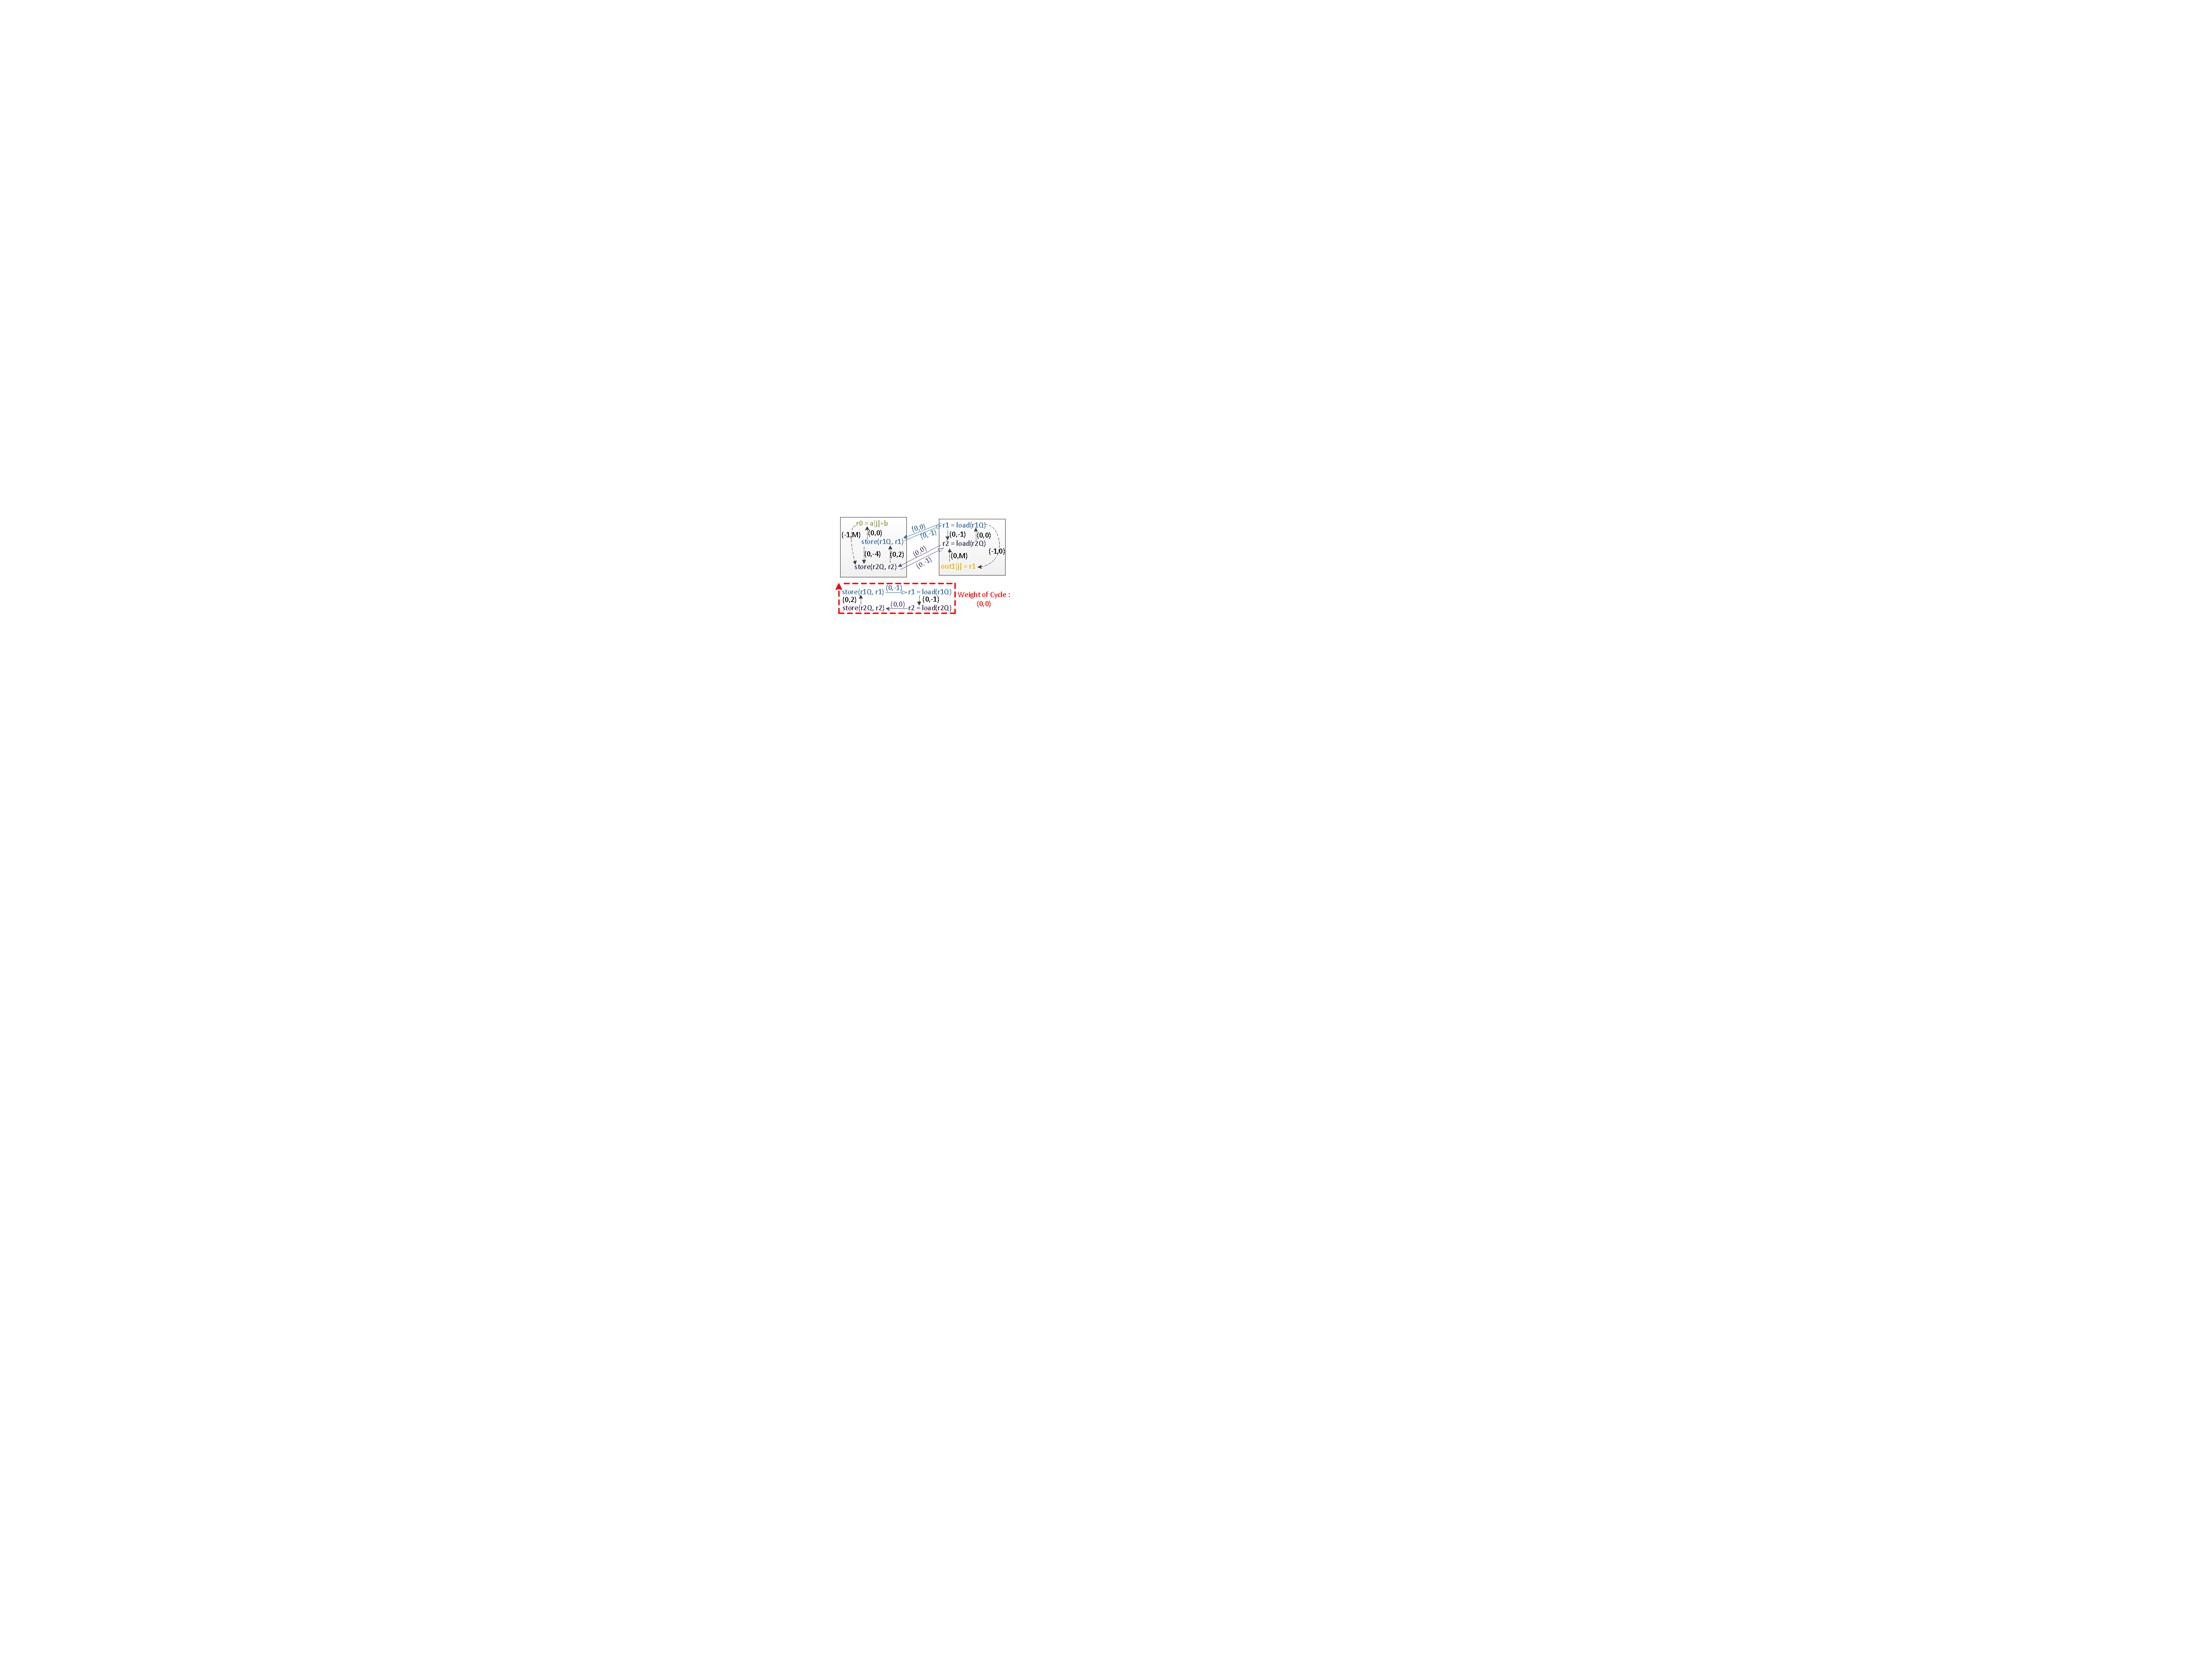
\includegraphics[width=0.8\linewidth]{fig/predGraphNew.pdf}
\caption{Precedence Graph for Process Network
\label{fig:predgraph}}
\end{center}
\vspace{-2.0em}
\end{figure}

Resolving
the deadlock involves choosing one of the $DepF$ edges
in the cycle and add enough slots (making the weight more negative)
such that the weight of the cycle gets a negative leading element. For our example in figure~\ref{fig:predgraph}, if the capacity of r1Q
is increased by 1, the weight on its corresponding $DepF$ becomes (0,-2). Consequently, the identified cycle in the figure would have
a total weight (0,-1), when the original artificial deadlock disappears.
In general, for every deadlock causing cycle, the $DepF$ edge whose channel has the smallest width can be selected for capacity expansion, so the cost of these extra slots is minimized. This heuristic does not necessarily produce an absolute
global optimal solution in the presence of multiple deadlock causing cycles, but suffices for our use cases.
\begin{comment}
Of course, as multiple non-negatively weighted cycles can be present simultaneously, the absolute global optimal solution would involve finding a set of $DepF$ edges, and minimize the aggregate cost of incrementing each for all cycles to be resolved. This is an NP hard problem
\end{comment}
%\subsection{Modelling Burst Mode Memory Access}






\begin{comment}

In~\cite{}, KPNs are 
categorized into strictly bounded, bounded and unbounded ones.
A KPN is strictly bounded if and only if any execution of of the network requires bounded space. It is bounded if and only if there are some
execution requiring bounded space while it is unbounded if and only if any
execution requires unbounded space. Methods to find bounds for communication channels
in KPNs were discussed in~\cite{}\cite{}. In general, whether a
KPN is bounded is undecidable~\cite{}, but for our process networks, which
are generated from sequential programs expressed in single static assignment
form, we can analyze the boundedness of the FIFO channels in various
scenarios.

To manifest the same behavior as the original sequential program, the generated network
needs to be bounded. This can be easily proven as a execution schedule constructed according to the original 

\end{comment}

\subsection{Deadlocks in Memory Accesses}
To exploit the memory bandwidth more efficiently, burst mode memory accesses are often used as well. Even though the memory ``process" does not block on reads, if the response data it sends to other normal processes is not consumed promptly, it can blocked on writes. 
The head-of-line blocking can then create a dependency cycle, resulting in a deadlock. Our precedence graph can be used to compute necessary buffer size to resolve this situation as well.

\begin{figure}[htp]
\begin{center}
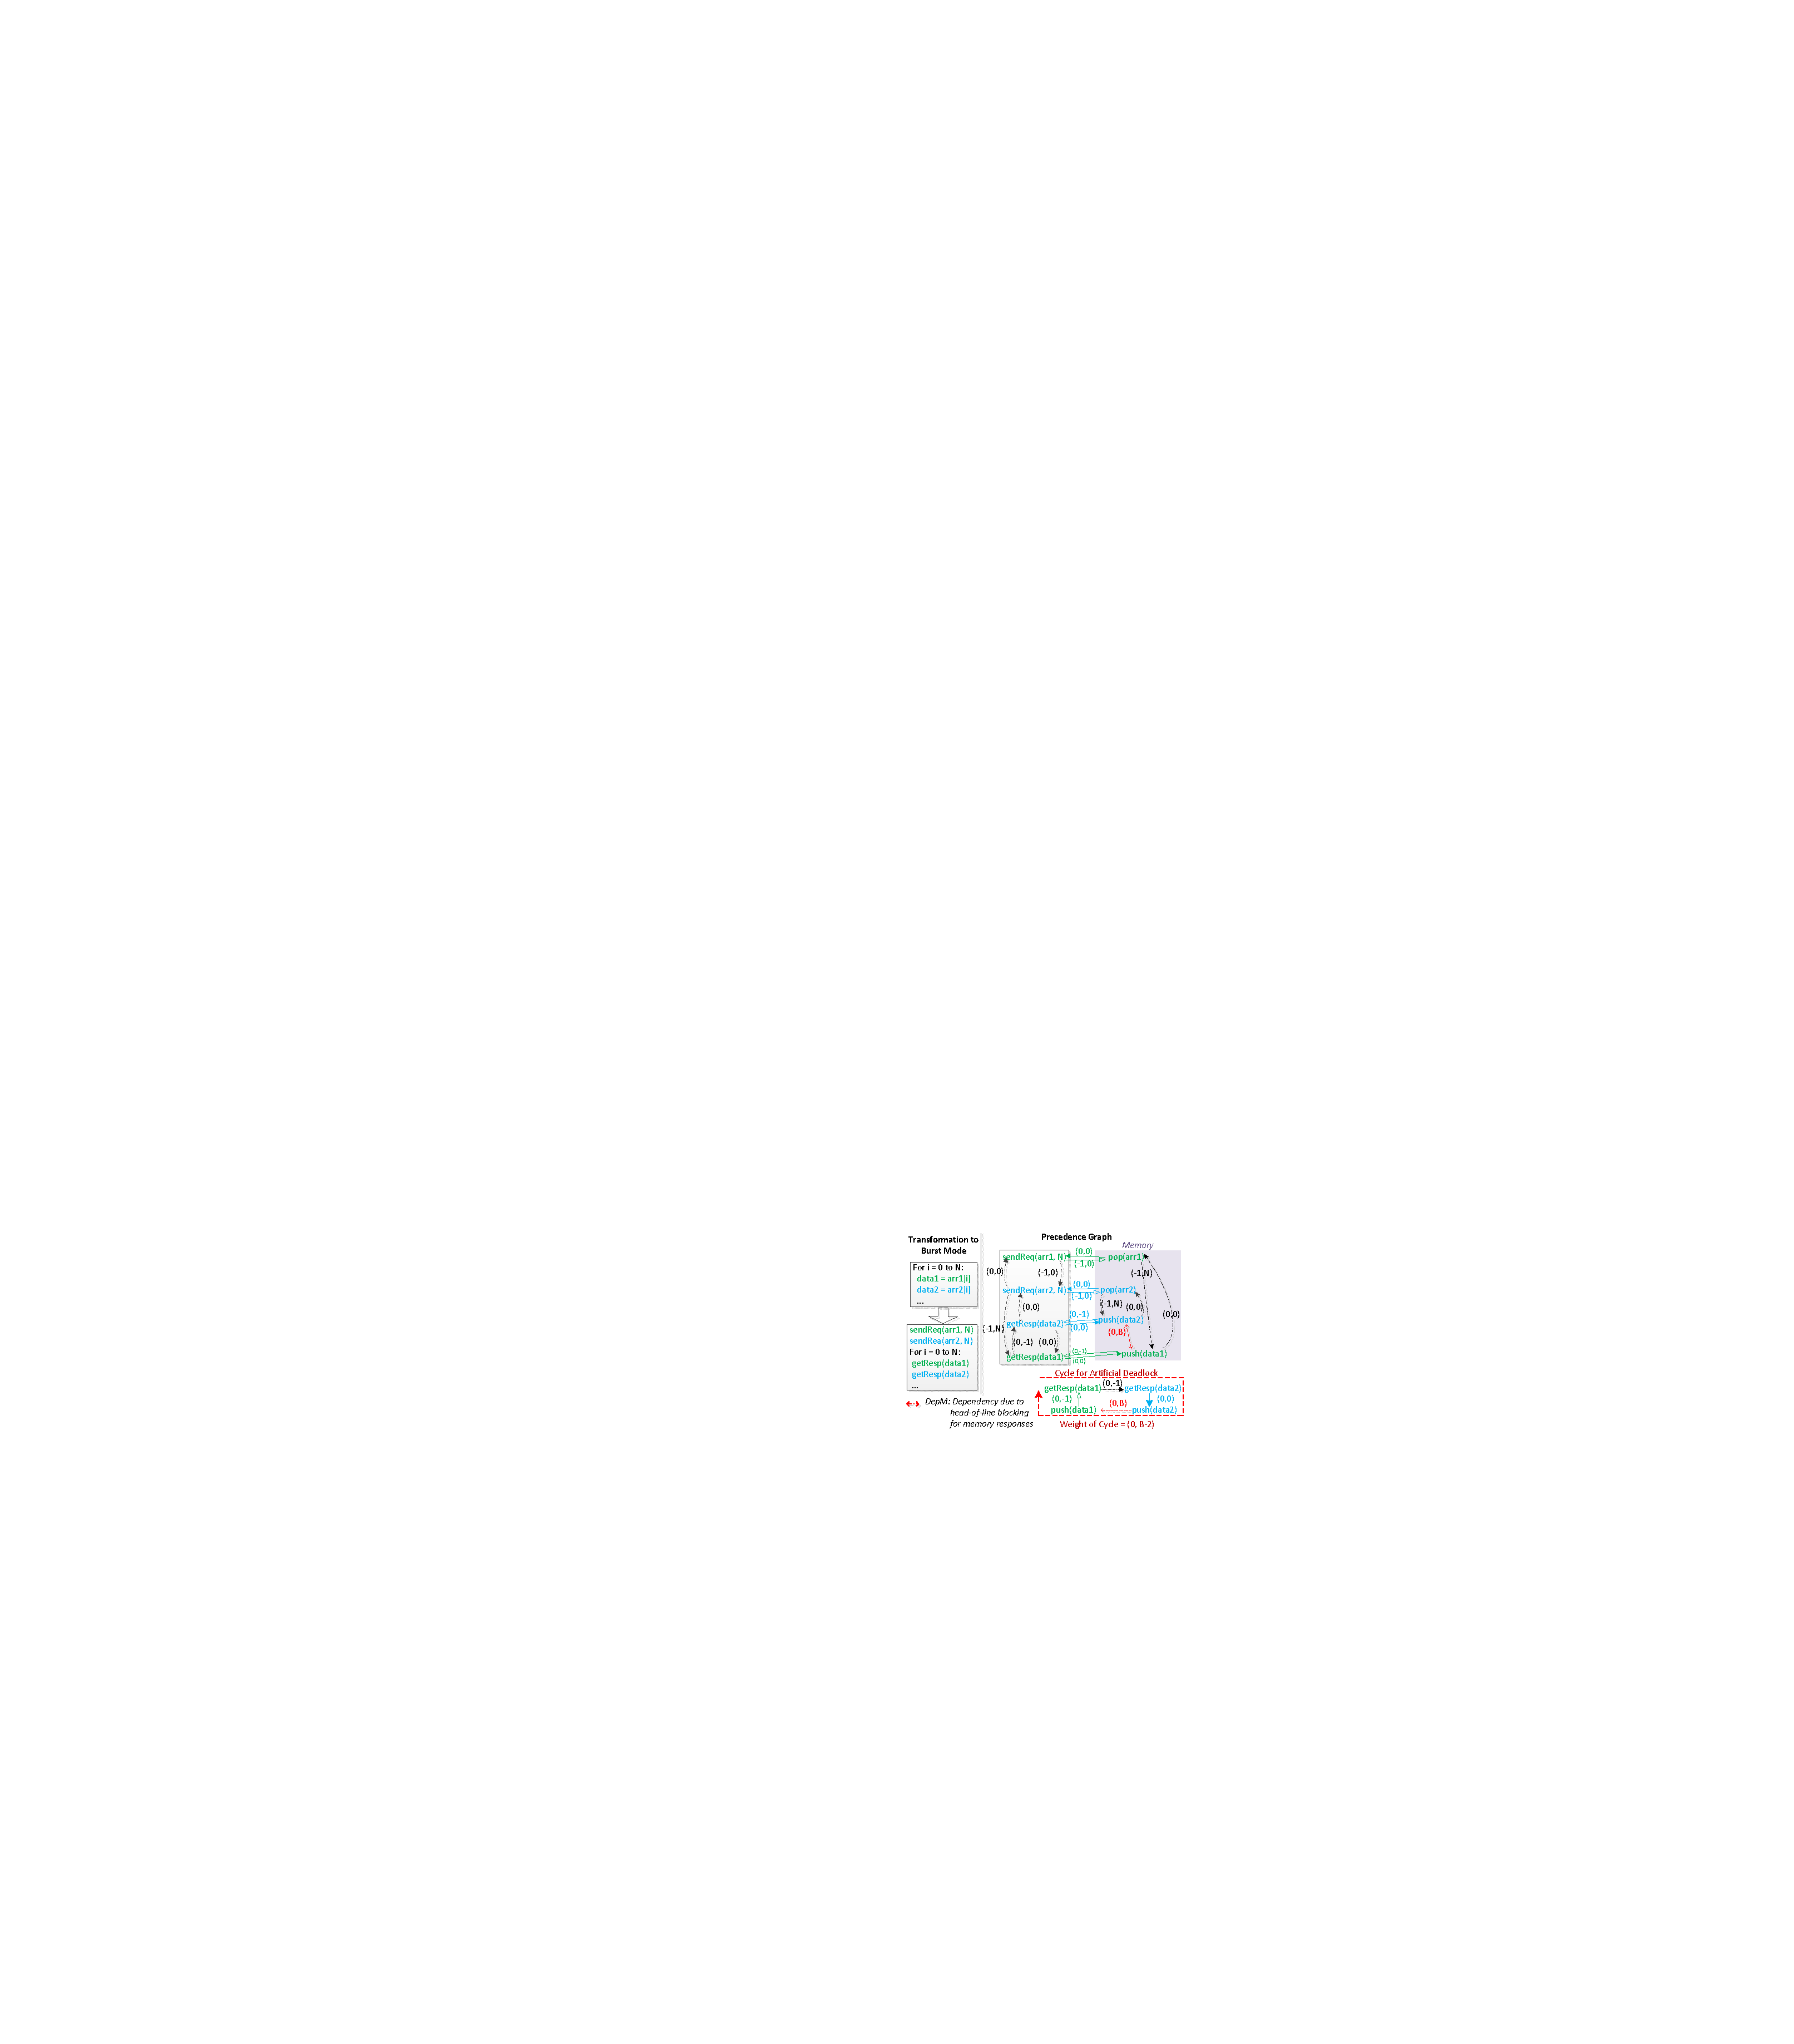
\includegraphics[width=1.05\linewidth]{fig/burstMem.pdf}
\caption{Precedence Graph for Process Network
\label{fig:memBurst}}
\end{center}
\vspace{-2.0em}
\end{figure}


Figure~\ref{fig:memBurst} illustrates how multiple burst mode memory accesses can
create a deadlock. The reaction of the memory is modelled by a pop action
responding to the incoming request, and a push action producing one response data token. Meanwhile, the sending of memory requests and receiving of responses are decoupled and assigned to different slots in the process schedule. This is often done in HLS because of the long latency of memory accesses.
For burst mode requests associated with a loop, the request sending is moved to outside of the loop as shown in the figure. The symbolic variable $B$ in the weight of the $DepM$ edge signifies how many tokens have to be consumed/buffered before the response for the next request ($data2$) become accessible for the response receiver. Assume the arbiter for the memory subsystem implements a policy which can potentially take in and serve multiple ($K$) consecutive requests from one stream, $B$ can be as big as $BurstSize_{max}*K$. 
In the case of a round-robin arbiter, $B = BurstSize_{max}$ and for our experiment platform which uses AXI bus protocol, this number is 256. With the precedence graph, we can easily compute that the buffering for the two memory response channels needs to be increased to $B$ for the deadlocks to be resolved.

\section{A Memory Centric Instruction Partitioning Algorithm}
\label{exampleAlgo}
So far, we have developed a framework to generate process network from a sequential program and a static analysis method to ensure sufficient FIFO spaces are allocated to prevent artificial deadlock. This section provides a concrete application of this
framework to generate high performance compute engines. The discussion in section~\ref{pre2} revealed the weakness of HLS generated FPGA accelerators, which
%is addressed by the partitioning algorithm developed in this section.
%The problem is 
can be
alleviated by decoupling memory accesses into different processes, each running its own schedule. Off-chip communication
and computation are naturally overlapped and the overall throughput of the compute
engine can be greatly improved.

More specifically, several factors are considered when the instructions are partitioned
to multiple sets. The starting point for the algorithm is a graph $G$ thoroughly annotated with various dependency information. The group of nodes which form dependency cycles are first identified. They are associated with loop carried dependencies and are the limiting factors for how aggressively loop iterations can be overlapped. The initiation
interval (II) of loops are dictated by the latency of these cycles.
As the communication channels will always add latency, it is undesirable to have
these cycles spanning multiple sets.
Secondly, we want to have memory operations separated from dependency cycles involving long latency computation, such that the stalls caused by cache misses no longer affect the computations running in another process. Lastly, to
localize the effects of stalls introduced by cache misses, the
number of memory operations in each set should be
minimized, especially when they address different parts of the
memory space.


%\subsection{The Partitioning Algorithm}
%\label{subsec:partalgo}
%In Algorithm~\ref{algo1}, the steps taken to achieve the aforementioned requirements are detailed.
The steps taken to achieve the aforementioned requirements are detailed,
In algorithm~\ref{algo1}.
The SCCs are collapsed into new nodes, which together with the original instruction nodes, are topologically
sorted. The obtained directed acyclic graph is traversed and a new set is created whenever a memory operation
or an SCC with long latency computation
is encountered. Here, long latency operations are those which cannot be completed within
one clock cycle, and
their categorization ultimately depends on the target frequency
of the final implementation on the FPGA. Currently, we
leverage Xilinx's Vivado HLS to generate latency estimate for
various compute operations. With a target clock frequency of
150MHz, for instance, floating point multiply takes four clock
cycles while a 32 bit integer addition can be completed within
a cycle. As Vivado HLS is eventually used as the backend for
our HDL generation, it provides accurate annotations for our
flow.




\begin{algorithm}[t]
  \caption{Instruction Partitioning}\label{algo1}
  \begin{algorithmic}[1]
  \Procedure{PartitionInstNodes}{G}%\Comment{G: CDFG of loop nests}
    \State SCCs $\gets$ allStronglyConnComps(G)
  \State DAG $\gets$ collapse(SCCs,G)
  \State topoSortedNodes $\gets$ topologicalSort(DAG)
  \State longSCCs $\gets$ getSCCWithLongOp(SCCs)
  \State memNodes $\gets$ findLdStNodes(G)
  \State memLongSCC $\gets$ LongSCCs $\cup$ memNodes
  \State allSets $\gets \{\}$
  \State curSet $\gets \{\}$
  \While{topoSortedNodes $\ne \emptyset$}
     \State curNode $\gets$ topoSortedNodes.pop()
     \State curSet $\gets$ curSet $\cup$ curNode
    
     \If{curNode $\in$ MemLongSCC}
     %\If{$curSubG \cap MemLongSCC \ne \emptyset$}
    \State allSets $\gets$ allSets $\cup$ curSet
    \State curSet $\gets$ \{\}
     %\EndIf
     \EndIf

     %\State $curSubG \gets curSubG \cup curNode$
     
  \EndWhile
  \State \Return allSets 
  %\State $OtherNodes = G - SCCs - MemNodes$
  %\State $SNodes\gets collapseSCC(G, SCCs)$
    %\State $i\gets 0$
    %\foreach{$r\not=0$}\Comment{We have the answer if r is 0}
  %\State $SGs\gets ClusterWithSeed(SCCs, MemNodes)$
  %\State $MGs\gets ClusterWithSeed(MemNodes, MemLongSCC)$
  %\State $OGs\gets ClusterWithSeed(OtherNodes, MemLongSCC)$
  %\State \Return $SGs \cup MGs \cup OGs$
  %\While{$SCCs \ne \emptyset$}
  %  \State $curSubG\gets \{\}$
  %  \State $curSCC\gets SCCs.pop()$
  %  \State $DFSCluster(curSCC,curSubG,MemNodes)$
  %  \State $Subgraphs\gets Subgraphs \cup curSubG$
  %\EndWhile
  %\While{$MemNodes \ne \emptyset$}
  %  \State $curSubG\gets \{\}$
  %  \State $curMem\gets MemNodes.pop()$
  %  \State $MemLongSCC\gets LongSCCs \cup MemNodes$
    %  \State $DFSCluster(curMem,curSubG, MemLongSCC)$
  %  \State $Subgraphs\gets Subgraphs \cup curSubG$
  %\EndWhile
  %\While{$OtherNodes \ne \emptyset$}
  %  \State $curSubG\gets \{\}$
  %  \State $curN\gets OtherNodes.pop()$
  %  \State $MemLongSCC\gets LongSCCs \cup MemNodes$
    %  \State $DFSCluster(curN,curSubG, MemLongSCC)$
  %  \State $Subgraphs\gets Subgraphs \cup curSubG$
  %\EndWhile
  %now do the otherNodes
  
    %\EndWhile\label{euclidendwhile}
    \EndProcedure
  %\Procedure{ClusterWithSeed} {$seeds$, $excludeSet$}
  %\State $subgraphs\gets \{\}$
  %\While{$seeds \ne \emptyset$}
    %\State $curSubG\gets \{\}$
    %\State $curN\gets seeds.pop()$
    %\State $DFSCluster(curN,curSubG, excludeSet)$
    %\State $subgraphs\gets subgraphs \cup curSubG$
  %\EndWhile
  
  %\State \Return $subgraphs$
  %\EndProcedure
  
  %\Procedure{DFSCluster} {$curN$, $curG$, $excludeSet$}
  %\If{$curN.isCovered()$}
  % \Return
  %\EndIf
  
  %\If{$curN \in excludeSet$}
  % \If{$curG \cap excludeSet \ne \emptyset$}
  %   \Return
  % \EndIf
  %\EndIf
  %\State $curG \gets curG \cup curN$
  %\State $curN.setCovered(true)$
  %\State $nextNodes\gets getDependents(curNode, DAG)$
  %\While{$nextNodes \ne \emptyset$}
  % \State $nextNode \gets nextNodes.pop()$
  % \State $DFSCluster(nextNode, curG, excludeSet)$
  %\EndWhile
  %\EndProcedure
  \end{algorithmic}
\end{algorithm}


\section{Experimental Evaluation}
\label{expEval}
To measure the benefits our approach, a set of benchmarks are pushed through our flow. The partitioning algorithm described in section~\ref{exampleAlgo} is applied together with the optimization step formulated in part~\ref{opt}. These benchmarks are kernels with non-regular control flow and memory access patterns. Their description is listed in table~\ref{tab:datasize}. 
As the input datasets are too big for on-chip buffers, and the memory accesses
being too irregular for simple DMA, these are cases where our flow can play a significant role
in improving the overall performance.

%Due to the presence of statically unknown off-chip memory accesses, these benchmarks are good cases where our algorithm can play a significant role in improving the overall performance. 

\begin{comment}
The benchmarks data footprints of the benchmarks
are listed in table~\ref{tab:datasize}

To evaluate the benefits of our approach, we took several benchmark kernels
and processed them with our flow. For sparse matrix vector (SpMV) multiply---our
first kernel---compressed sparse
row (CSR) format is used to store the matrix, where the loads of the floating
point numbers to be multiplied depend on the data in an index array.
The next two kernels, Knapsack and Floyd-Warshall, are both dynamic programming problems. The memory
addresses to be accessed are derived from the results of computation.
Our final kernel, Depth first search (DFS), is a widely used graph algorithm. The benchmarked version
operates on pointer based data structure and uses a stack. All these kernels
are sequential code with non-regular control flow and memory access patterns. 
The input dataset for each benchmark, as described by 
Table~\ref{tab:datasize}, is also too big to fit entirely on chip. 
Due to the presence of statically unknown off-chip memory accesses, these benchmarks are good cases where our algorithm can play a significant role in improving the overall performance.
On the other hand, for problems where the entire data set can be buffered on chip or when the memory access patterns are regular, our approach would offer little
performance advantage over the conventional DMA+accelerator approach~\cite{vivado_hls:appnoteMMult}.
\end{comment}

%\renewcommand{\tabcolsep}{0.5pt}

%\vspace{-0.7em}
\begin{table}[htbp]
\caption{Benchmark Descriptions}
%\vspace{-1.2em}
\scriptsize
\centering
\begin{tabular}{| c | c | c | }
  \hline            
  
 %\multirow{2}{*}{\bf Benchmark}   &   \multirow{2}{*}{Description of Input Data} & \multirow{2}{*}{Total Size of Input Data}\\
% {\bf Benchmark}& {Description }      & {Input Data Size}  \\
  \multirow{2}{*}{\textbf{Benchmark}}& \multirow{2}{*}{\textbf{Description}}  & \multirow{2}{*}{\textbf{Data Size}}  \\
%\cline{2-3}                                                                                                                                                    
  &       &   \\
  
  \hline            
                                                                                     
\hline
\multirow{2}{*}{}Floyd-& {Graph Algo. with Dynamic Programming}  & \multirow{2}{*}{$\approx$ 8 MB}  \\
%\cline{2-3}                                                                                                                                                    
 Warshall & Memory Accesses Depend on Computation       &   \\
%\cline{2-3}                                                                          
\hline                                                                                                           
\multirow{2}{*}{Knapsack}& Optimization with Dynamic Programming &\multirow{2}{*}{$\approx$ 5 MB}  \\
%\cline{2-3}                                                                                                                                                    
  &Memory Accesses Depend on Computation       &   \\
%\cline{2-3}                                                             
\hline
\multirow{2}{*}{}Depth-First&  Number of Nodes = 4000 & \multirow{2}{*}{$\approx$ 3 MB}  \\
%\cline{2-3}                                                                                                                                                    
 Search & Number of Neighbors per Node = 200       &   \\
%\cline{2-3}                                                                        
\hline            
\multirow{2}{*}{}SpMV& Matrix in Compressed Row Storage & \multirow{2}{*}{ $\approx$ 16 MB}  \\
%\cline{2-3}                                                                                                                                                    
 Multiply &Indirect Memory Addressing      &  \\
%\cline{2-3}                                                                                                             
                                
  \hline      
  
\end{tabular}
\label{tab:datasize}
\end{table}



The FPGA device used for our evaluation is the Zynq-7000 XC7Z020 FPGA
SoC from Xilinx, installed on the ZedBoard evaluation platform. The SoC contains two parts: an ARM-processor based processing
system (PS), and the programmable logic (PL). 
The baseline for our evaluation is the performance of each software kernel running
on the ARM core in the PS. 
The core is an out-of-order, dual-issue hard
processor running at 667MHz. The Zynq platform also provides two
options for the accelerators in PL to access the main memory subsystem: 
through the accelerator coherence port (ACP), or the high performance (HP) port. 
The former connects to the snoop control unit in the processing system and 
thus uses/modifies the processing system's on chip cache. The HP port connects
directly to the memory controller, thus often imposes a longer round-trip latency
for data requests.
\begin{comment}
which necessitates the flushing of cache lines 
by the processor if cached memory is accessed by the accelerator.
In either case, if memory states are also buffered in the PL with caches, they 
need to be explicitly pushed to the processing system side after the accelerator finishes running. 
As both the ACP
and the HP are slave ports, they provide no mechanisms to extract data from the programmable logic
when the ARM processor is running. The interaction between the generated accelerators
and the main pieces of the FPGA SoC is shown in figure~\ref{fig:ippf}.
\end{comment}

\begin{comment}
\begin{figure}[htp]
\begin{center}
\includegraphics[width=0.9\linewidth]{fig/system.pdf}
\caption{Implementation of Dataflow Accelerators in FPGA SoC  
\label{fig:ippf}}
\end{center}
%\vspace{-1.0em}
\end{figure} 
\end{comment}

\begin{figure*}[htp]
\begin{center}
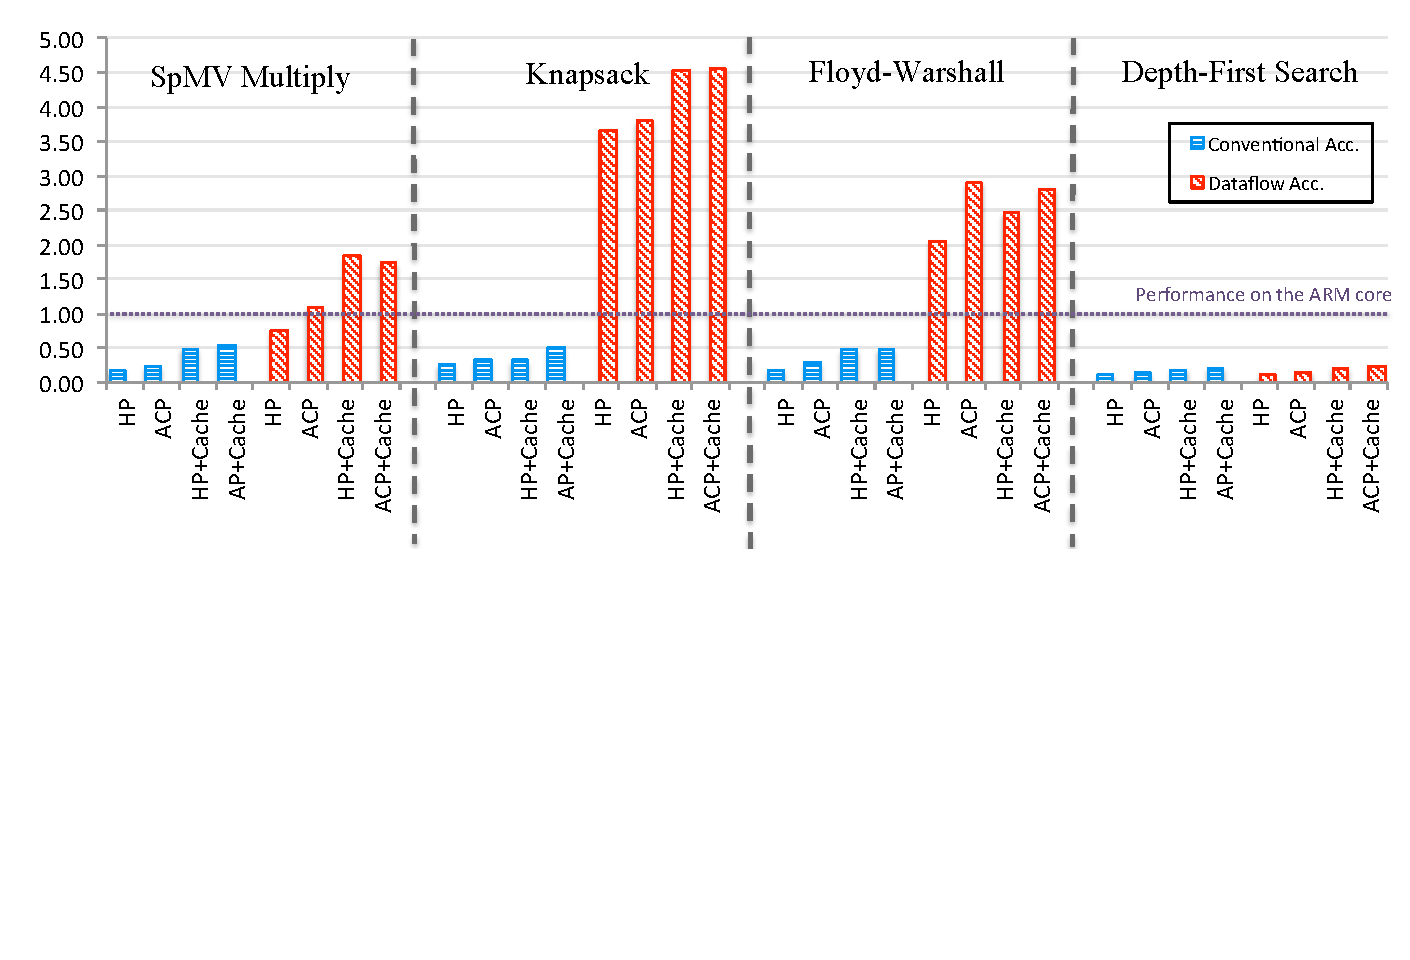
\includegraphics[width=0.95\linewidth]{fig/perf.pdf}
\caption{Performance of Conventional Accelerators and Accelerator Networks, normalized to the hard ARM core. Implementations with caches use
Xilinx System Cache IP, configured to be 64KB and 2-way associative   
\label{fig:acpraw}}
\end{center}
\vspace{-2.7em}
\end{figure*} 


In our study, Vivado HLS, a state-of-the-art high level synthesis tool provided by Xilinx,
is used to generate the accelerators for the original sequential code, as well as the processes created by our flow. With the target clock period set to 
8ns during HLS, the tightest timing constraints post place \& route implementations managed to meet range from 111 to 150MHz. 
All design points shown in this section 
use the highest achievable frequency as the actual operating clock frequency. 
%\vspace{-1.0em}
\subsection{Performance Comparisons}
In figure~\ref{fig:acpraw}, 
performance of the different implementations are presented. 
Conventional accelerators and dataflow accelerators with different memory subsystem
configurations are compared. All the numbers are normalized to the baseline.

In all four benchmarks, conventional accelerators directly generated from software kernels using the HLS flow
actually have lower performance than the hard processor. Even with
on-PL caches, 
these accelerators only manage to achieve throughput less than 50\% that of the baseline. 
The superscalar, 
out-of-order ARM core is capable of exploiting instruction level parallelism to a good extent 
and also has a high performance on-chip cache.
The additional parallelism extracted by the HLS tool is evidently not enough
to compensate for the clock frequency advantage the hard processor core has over the programmable logic and the longer data access
latency from the reconfigurable array. 

With our methodology, the accelerator networks generated 
are rather competitive against the hard processor, even
without a reconfigurable cache. For SpMV multiply, knapsack and Floyd-Warshall, when the networks are directly connected to the memory through the ACP, 
the average performance is 2.3x that of the baseline---representing
an 8.4x gain over the conventional accelerators.
Upon the addition of caches,  
the average runtime of the accelerator networks was reduced by 18.7\%,  while that of the conventional
accelerators was cut by 45.4\%. The gap between their performance is thereby reduced from 8.4 to 5.6 times. This difference in improvement is due to conventional accelerators' sensitivity to the latency of data accesses, which is also manifested by its performance degradation of 40\% when the uncached HP port is used instead of ACP. 

\begin{comment}
It is also apparent that our approach has its limitations, as demonstrated by its ineffectiveness in the 
depth first search benchmark.
The kernel performs very little computing but lots of memory accesses.
The use of a stack in DFS also creates a dependence cycle through the memory
and consequently, the performance is fundamentally limited by the latency of memory access.
Thus there were only small differences between the performance of the conventional accelerator and the dataflow accelerator. Besides, the memory access pattern
does not provide many opportunities for optimizations. As a result, both accelerators achieves performance far below that of the baseline.
\end{comment}

Overall, for kernels suitable for FPGA acceleration, there is a significant performance advantage in using
an intermediate dataflow architectural template. If we compare the best results achieved with the
dataflow accelerators to that of the conventional accelerators, we see improvement
of 3.3 to 9.1 times, with an average of 5.6. 
%This performance advantage translates to energy savings as well, as illustrated in the next section.





%\subsection{Area and Energy Comparison}
%\vspace{-1.0em}
\subsection{Area comparison}
To quantify the impact of our proposed methodology on area, 
we have compared the FPGA resouce usage of conventional accelerators and
the dataflow accelerators.
Table~\ref{tab:areacom} shows the results, 
where each acclerator is complemented with two different memory subsystem configurations.
\renewcommand{\tabcolsep}{0.5pt}
\begin{table}[htbp]
%\vspace{-1.2em}
\caption{Resource Usage of Accelerators.}
%\vspace{-1.2em}
\scriptsize
\centering
\begin{tabular}{| c | c | c | c | c | c | c | c| }
  \hline            
  \multirow{2}{*}{} &  &   \multicolumn{3}{c|}{\bf ACP  } & \multicolumn{3}{c|}{\bf ACP + 64KB Cache }   \\
 \cline{3-8} 
 {\bf Benchmark}   &    & LUT& FFs& BRAM & LUT &   FFs      & BRAM    \\
  %
  %                 & LUT &FFs&  BRAM &  LUT &   FFs      & BRAM   \\
  \hline            
  \hline            
\multirow{3}{*}{}&Con.Acc  & 9873 &9116 &10 & 7918 & 6792 & 21  \\
\cline{2-8}                                                                                                                                                    
SpMV &Dataflow Acc       & 8577 & 8837& 10 & 6718  &6788 & 21\\
\cline{2-8}                                                                                                             
    Multiply   &\% change & -13.1 &-3.1 & 0 & -15.2  & -0.1 & 0  \\
  \hline                                                                                                           
\multirow{3}{*}{}&Con.Acc  & 7672 &7490 &8 & 6573 & 5885 & 21  \\
\cline{2-8}                                                                                                                                                    
Knapsack &Dataflow Acc       & 8089 & 8787& 8 & 6970  &7256 & 21\\
\cline{2-8}                                                                                                             
       &\% change & +5.4 &+17.3 & 0 & +6.0  & +23.3 & 0  \\
  \hline                                                                                                           
\multirow{3}{*}{}&Con.Acc  & 2491 &3528 &0 &3806  &4629  &19   \\
\cline{2-8}                                                                                                                                                    
Floyd- &Dataflow Acc       & 7659 &7210 &0  &8995  &8309 &19 \\
\cline{2-8}                                                                                                             
 Warshall      &\% change &+207.5  &+104.3 & 0 & +104.4  & +79.5  & 0  \\
  \hline                                                                                                           
\multirow{3}{*}{}&Con.Acc  & 4810 &4929 &4 & 4931 & 4594 & 21  \\
\cline{2-8}                                                                                                                                                    
DFS &Dataflow Acc       & 8509 & 7813& 4 & 7436  &6298 & 21\\
\cline{2-8}                                                                                                             
       &\% change & +76.9 &+58.5 & 0 & +50.8  & +37.1 & 0  \\
  \hline                                                                                                           

\end{tabular}
\label{tab:areacom}
\end{table}


The difference in area between the dataflow accelerators and the conventional accelerators is effected by
two factors.  
When the dataflow architectural template is used, there are always additional costs associated with the communication channels. Meanwhile, as
the original programs are partitioned into subgraphs and separately turned into hardware, the depth of the internal 
pipeline in each module is reduced, resulting in area savings. 
%as compared to the instantiation
%of the same set of operators in conventional accelerators. 
%For instance,
%in our motivating example, the initiation interval of the inner loop is 
%determined by the floating point multiply. The loop counter, which is
%another SCC in our dataflow, will also need
%to be synchronized to the same schedule, which necessitate insertion of
%additional pipeline stages. 
The overall change therefore depends on which factor plays a larger role, and is 
ultimately application specific. 




\section{Related Work}
\label{relatedwork}
Parallelizing sequential programs by transforming them to process networks was attempted in multiple past projects. The Compaan flow~\cite{mat2pn} takes Matlab code and generates
process networks. ESPAM~\cite{4378214}\cite{c2stream}, on the otherhand, uses sequential C as the input language and also provides an efficient method to compute the needed FIFO size. They also have extension for implementing the PN on FPGAs. However, the targets of their flow are highly regular kernels with statically analyzable memory access patterns, which are quite different than the benchmarks we have applied our framework to. 

For FIFO sizing and deadlock resolution in process networks, many approaches were proposed over the years. Most of these involves monitoring execution and dynamically incrementing FIFO sizes when deadlock occurs~\cite{parks1995bounded}\cite{Geilen:2003:REK:1765712.1765736}\cite{4217338}, 
due to the infeasibility of analyzing deadlock for generic process networks at compile time. In our flow, we ensure, by construction, each FIFO is only read/written by a single instruction in each process, a graph based static analysis framework can be used to find the needed FIFO sizes.

Finally, HLS for FPGAs are being active developed in both industry~\cite{tools:vivadohls} and academia~\cite{tools:legup}. Researchers
have also tried different programming paradigms~\cite{Lebedev:2010:MMA:1935936.1936078}
to expose greater amount of parallelism to HLS. Our work complements
HLS by providing a higher level transformation infrastructure which, when
used appropriately, can significantly improve the quality of the generated compute engine.






\section{Conclusions}
\label{conclude}
This paragraph will end the body of this sample document.
Remember that you might still have Acknowledgments or
Appendices; brief samples of these
follow.  There is still the Bibliography to deal with; and
we will make a disclaimer about that here: with the exception
of the reference to the \LaTeX\ book, the citations in
this paper are to articles which have nothing to
do with the present subject and are used as
examples only.
%\end{document}  % This is where a 'short' article might terminate

%ACKNOWLEDGMENTS are optional

\begin{comment}
\section{Acknowledgments}
This section is optional; it is a location for you
to acknowledge grants, funding, editing assistance and
what have you.  In the present case, for example, the
authors would like to thank Gerald Murray of ACM for
his help in codifying this \textit{Author's Guide}
and the \textbf{.cls} and \textbf{.tex} files that it describes.
\end{comment}


%
% The following two commands are all you need in the
% initial runs of your .tex file to
% produce the bibliography for the citations in your paper.
\bibliographystyle{ieeetr}
\bibliography{sigproc}  % sigproc.bib is the name of the Bibliography in this case
% You must have a proper ".bib" file
%  and remember to run:
% latex bibtex latex latex
% to resolve all references
%
% ACM needs 'a single self-contained file'!
%
%APPENDICES are optional
%\balancecolumns
\begin{comment}
\appendix
%Appendix A
\section{Headings in Appendices}
The rules about hierarchical headings discussed above for
the body of the article are different in the appendices.
In the \textbf{appendix} environment, the command
\textbf{section} is used to
indicate the start of each Appendix, with alphabetic order
designation (i.e. the first is A, the second B, etc.) and
a title (if you include one).  So, if you need
hierarchical structure
\textit{within} an Appendix, start with \textbf{subsection} as the
highest level. Here is an outline of the body of this
document in Appendix-appropriate form:
\subsection{Introduction}
\subsection{The Body of the Paper}
\subsubsection{Type Changes and  Special Characters}
\subsubsection{Math Equations}
\paragraph{Inline (In-text) Equations}
\paragraph{Display Equations}
\subsubsection{Citations}
\subsubsection{Tables}
\subsubsection{Figures}
\subsubsection{Theorem-like Constructs}
\subsubsection*{A Caveat for the \TeX\ Expert}
\subsection{Conclusions}
\subsection{Acknowledgments}
\subsection{Additional Authors}
This section is inserted by \LaTeX; you do not insert it.
You just add the names and information in the
\texttt{{\char'134}additionalauthors} command at the start
of the document.
\subsection{References}
Generated by bibtex from your ~.bib file.  Run latex,
then bibtex, then latex twice (to resolve references)
to create the ~.bbl file.  Insert that ~.bbl file into
the .tex source file and comment out
the command \texttt{{\char'134}thebibliography}.
% This next section command marks the start of
% Appendix B, and does not continue the present hierarchy
\section{More Help for the Hardy}
The sig-alternate.cls file itself is chock-full of succinct
and helpful comments.  If you consider yourself a moderately
experienced to expert user of \LaTeX, you may find reading
it useful but please remember not to change it.

\end{comment}
%\balancecolumns % GM June 2007
% That's all folks!
\end{document}
